\section{Timing of photons coming from $^{10}$C background}

Background from $\Cten$ could be significant at a shallow detector depth.
Here we discuss separation of $\vbb$-decay events from $\Cten$ background using 
differences in PE arrival time distributions between signal and background events.
$\Cten$ decays to a positron and a gamma. The positron produces scintillation light 
along its trajectory of a few mm before it stops and anihillates into two 0.511~keV 
gammas. The kinetic energy of the positron from $\Cten$ is smaller than total kinetic
energy of the electrons from $\vbb$-decay. Therefore the amount of scintillation 
light produced at the primary vertex by the positron is smaller than the amount of 
scintillation light produced by electrons in $\vbb$-decay. The scintillation light from 
gammas is produced at several secondary verticies along gammas trajectories of $\sim X0$. 
This results in a PE arrival time distribution for $\Cten$ events that is shifted towards 
longer times with respect to the $\vbb$-decay events.

This time shift would be valid for any backround whith a positron in the final state. In 
$\Cten$ this shift is increased because $\Cten$ decays via an excited state of $^{10}$B(718),
which has a half-life time of $\sim$1~ns, so that 0.718~MeV gamma has a delay with respect
to the positron that is detectable by photo-detectors with $\sim$100~ps time resolution.

In the following we assess the separation between $\vbb$-decay and $\Cten$ events due to the 
time shift in the PE arrival time distribution. We discuss requirements on the primary vertex 
reconstruction resolution and the time resolution of the photo-detectors.

Typical energy deposition by $^{10}$C events is shown in
Fig.~\ref{fig:Edep_C10}. Vertical lines indicate Q-value of $\Te$ and 
$\pm$10\% region around Q-value. In order to include detector energy resolution 
effects we consider $\Cten$ events in this region, which is 2.276~MeV - 2.782~MeV.
\footnote{Everywhere below we refer to this energy range for $\Cten$ events unless 
stated otherwise}


\begin{figure}[h]
  \centering
  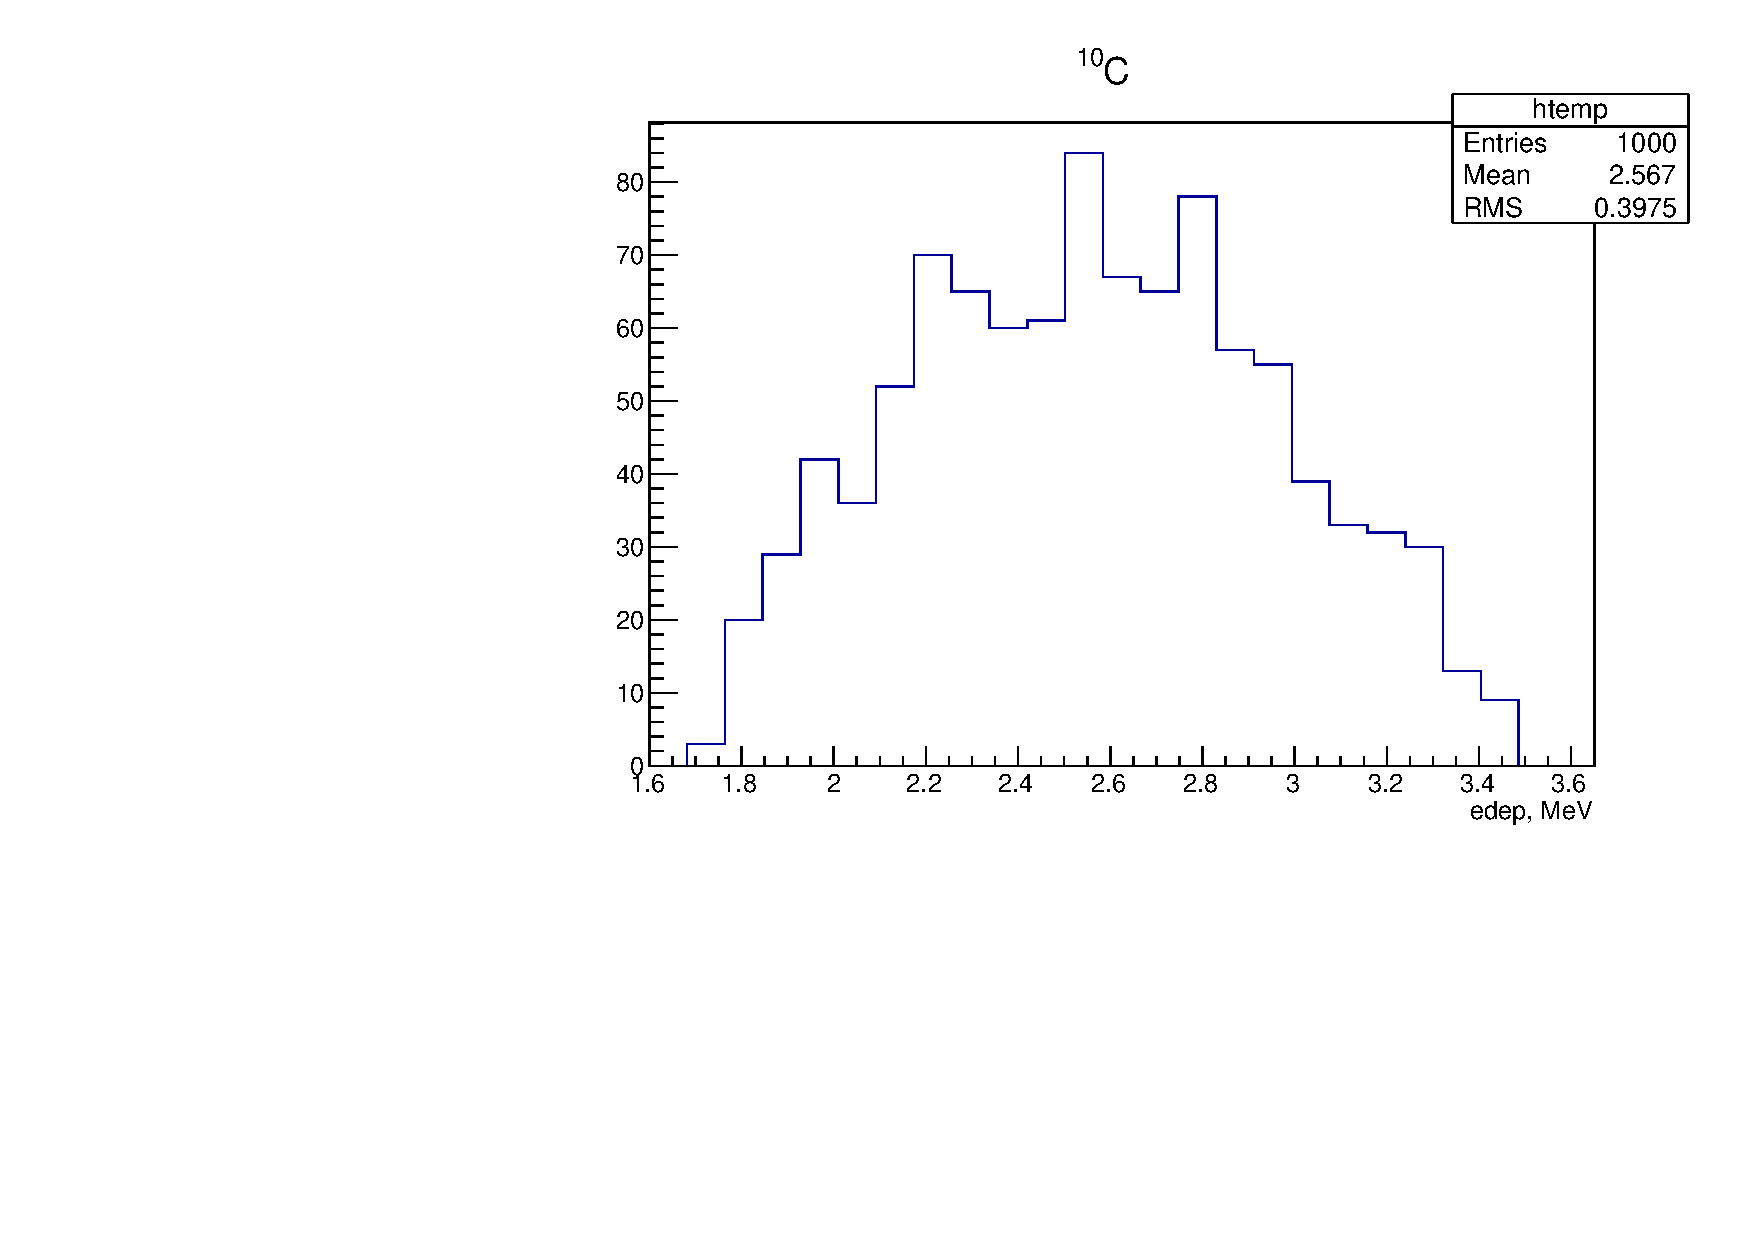
\includegraphics[width=0.95\textwidth]{hEdep_C10.pdf}
  \caption{$^{10}$C energy deposition in the detector. Simulation of 10000 events
  produced at the center of the detector. Solid red line at 2.529~MeV indicates $\Te$ 
  Q-value. Dashed red lines at 2.276~MeV and 2.782~MeV show $\pm$10\% region around 
  Q-value.}
  \label{fig:Edep_C10}
\end{figure}

Since 98\% of $^{10}$C decays through an excited state of $^{10}$B(718), 
which has a half-life time of $\sim$1~ns, the majority of $^{10}$C events have 
a prompt positron accompanied by a delayed 0.718~MeV gamma. The positron energy
has to be 0.79~MeV for an event to have energy deposition equal to Q-value of
$\Te$ $\vbb$-decay.

The positron from $\Cten$ on average travels 4~mm before it stops and anihilates
producing two 0.511~MeV gammas. Those gammas then interact in the scintillator via 
Compton scattering and photo-electric effect along while they loose their energy
over $\sim X_0$ distance. Therefore light emmited in $\Cten$ events originates from
several clusters that are spread over $\sim X_0$. Significant fraction of the 
early PE would be due to primary positron cluster. Because the positron has smaller 
kinetic energy than kinetic energy of electrons from $\vbb$-decay the amount of early 
PE is smaller for $\Cten$ events. Delayed 0.718~MeV gamma in some of $\Cten$ events 
also result in a delay in the photon arrival time with respect to $\vbb$-decay events.

Figure~\ref{fig:Arrival_time_C10_overlaid} compares PE arrival times between 
$\vbb$-decay and $\Cten$ events. To separate the time shift due to smaller kinetic 
energy of the positron and due to the decay via a long lived $^{10}$B(718) state we 
include simulation of prompt $\Cten$ decays. The prompt $\Cten$ is a simplified simulation 
where a positron is simultaneously produced with a 0.718~MeV gamma. The difference between
prompt $\Cten$ and $\vbb$-decay is caused by presence of a positron and this 
difference is typical on event by event level. An additional difference due to delayed
gamma shown in Fig.~\ref{fig:Arrival_time_C10_overlaid} is an average effect over 1000 events. 
Significant variations are possible on event by event level since $^{10}$B(718) decay 
time is exponential.

\begin{figure}[h]
  \centering
  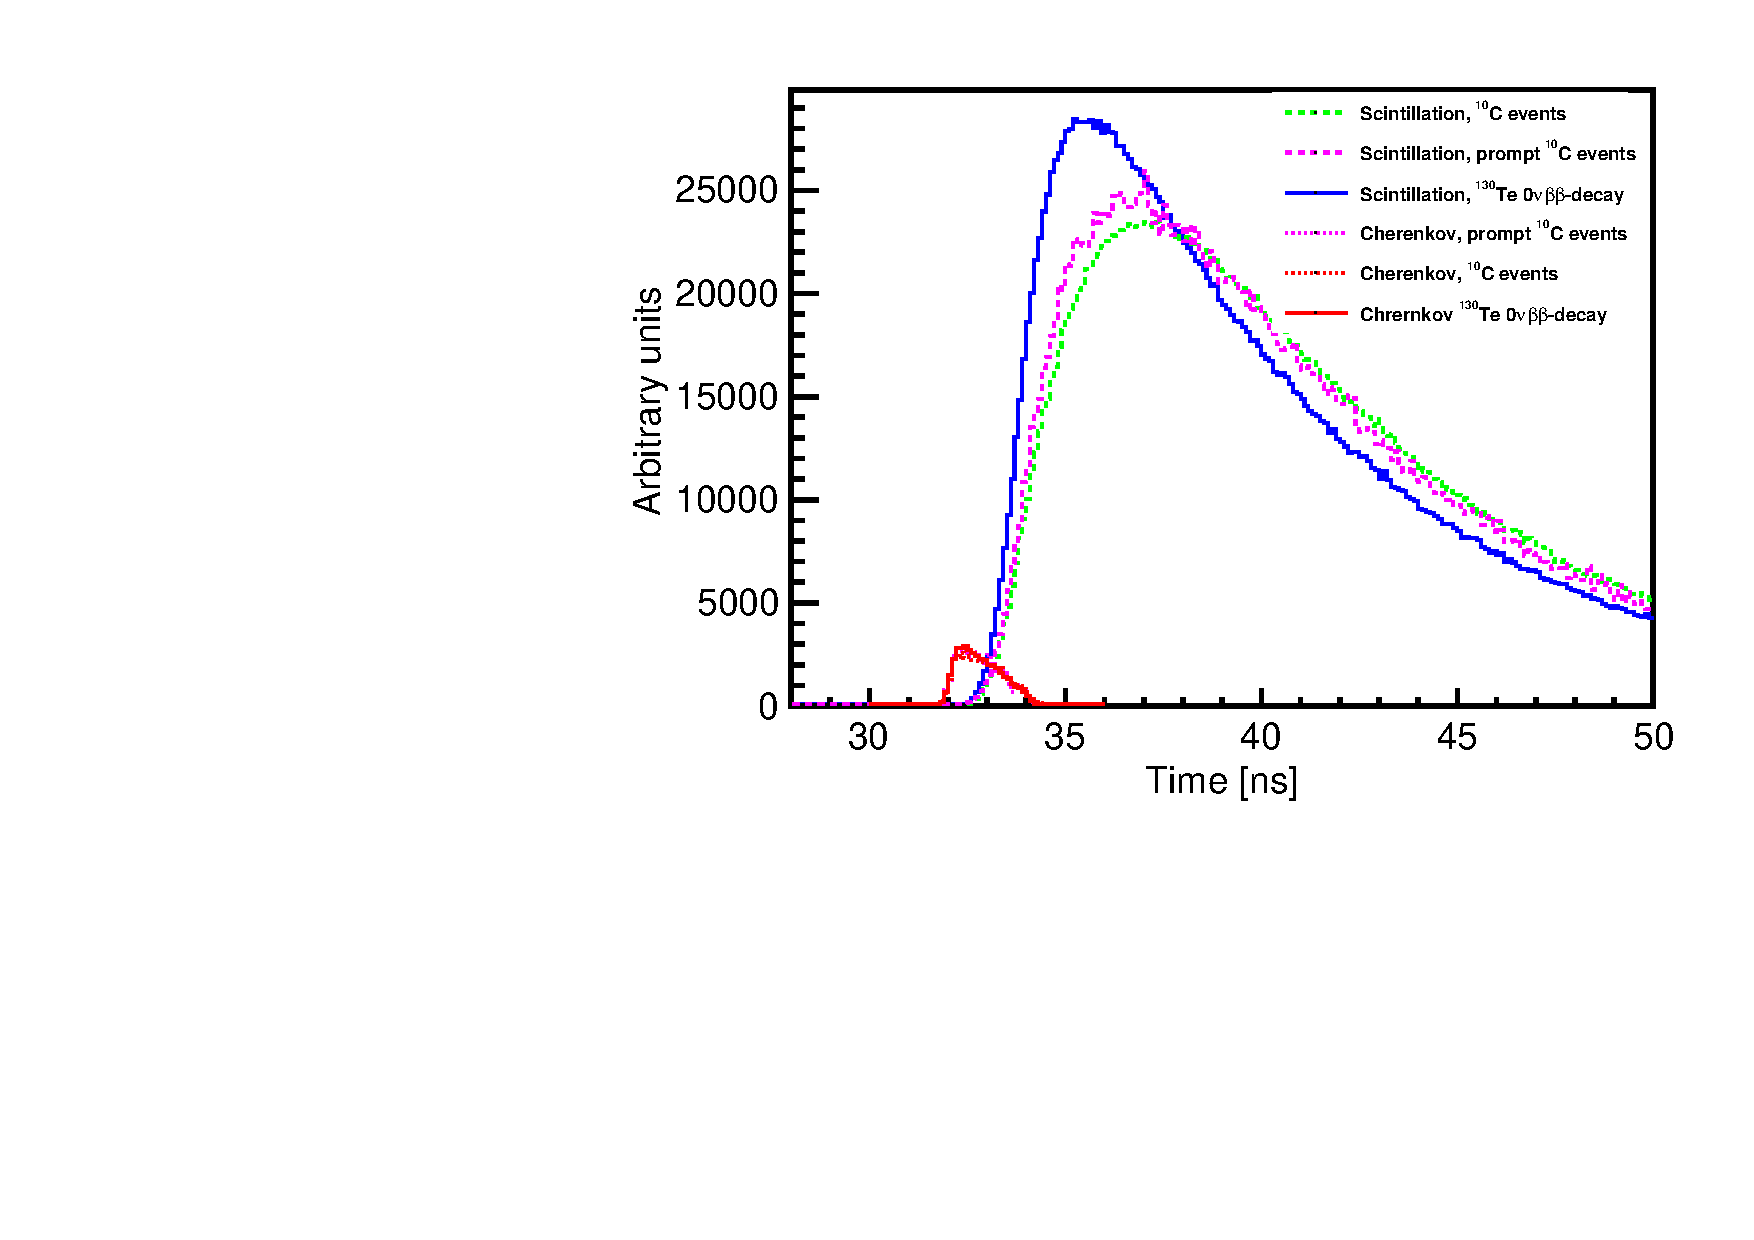
\includegraphics[width=0.95\textwidth]{hT_Te130vsC10_overlaid_v2.pdf}
  \caption{Photo-electron (PE) arrival times after application of the
    photo-detector transit time spread (TTS) of 100~ps for the
    simulation of 1000 0{\nbb} decay events of $^{130}$Te (\emph{solid
      lines}) and $^{10}$C (\emph{dotted lines}) events at the center
    of the detector. Cherenkov and scintillation components are are normalized for 
    for shape comparison.}
\label{fig:Arrival_time_C10_overlaid}
\end{figure}

As can be seen from Fig.~\ref{fig:Arrival_time_C10_overlaid} there is a noticable difference
in the shape of PEs arrival time distribution between $\vbb$-decay and $\Cten$ events. A fit
to a template shapes can be used to discriminate between signal and background. In this study,
to distinguish between $\vbb$-decay and $\Cten$ events we count total number of PEs in the
early light sample. 

Two definitions of the early light sample are used. First, for central events, where we assume 
perfect knowledge of the primary vertex location, the early light sample is defined as PEs 
with arrival time t$<$33.5~ns. Second, for a more realistic scenario, where the vertex is uniformly 
distributed within the fiducial volume and the uncertainty on the vertex position reconstruction
is taken into account, the early light sample is defined as PEs with $\Delta T=T_{measured} - 
T_{predicted}<$1~ns, where $T_{measured}$ is measured arrival time and $T_{predicted}$
is predicted arrival time based on the primary vertex location: 
$T^{predicted} = |r_{hit} - r_{vtx}|/v_{phot}$, where $v_phot = c/1.53$ is avearge photon velocity
in the scintillator, $r_{hit}$ is the position of the PE on the photo-detector, and $r_{vtx}$ is the
reconstructed position of the primary vertex.


Numbers of Cherenkov and scintillation PEs in early light samples for $\vbb$-decay and 
$\Cten$ central events are shown in Fig.~\ref{fig:NPhotDist_C10}. Perfect reconstrution of the 
primary vertex is assumed and a time cut of 33.5~ns is used to define early light sample. 
Distributions of total number of PEs in the early light sample for $\vbb$-decay and $\Cten$ events
normalized to the same number of simulated events are overlaid in Fig.~\ref{fig:NPhot_compare_central}.
We conclude that counting PEs that arrive early provides effective separation between signal and
background.


\begin{figure*}[ht]
  \centering
  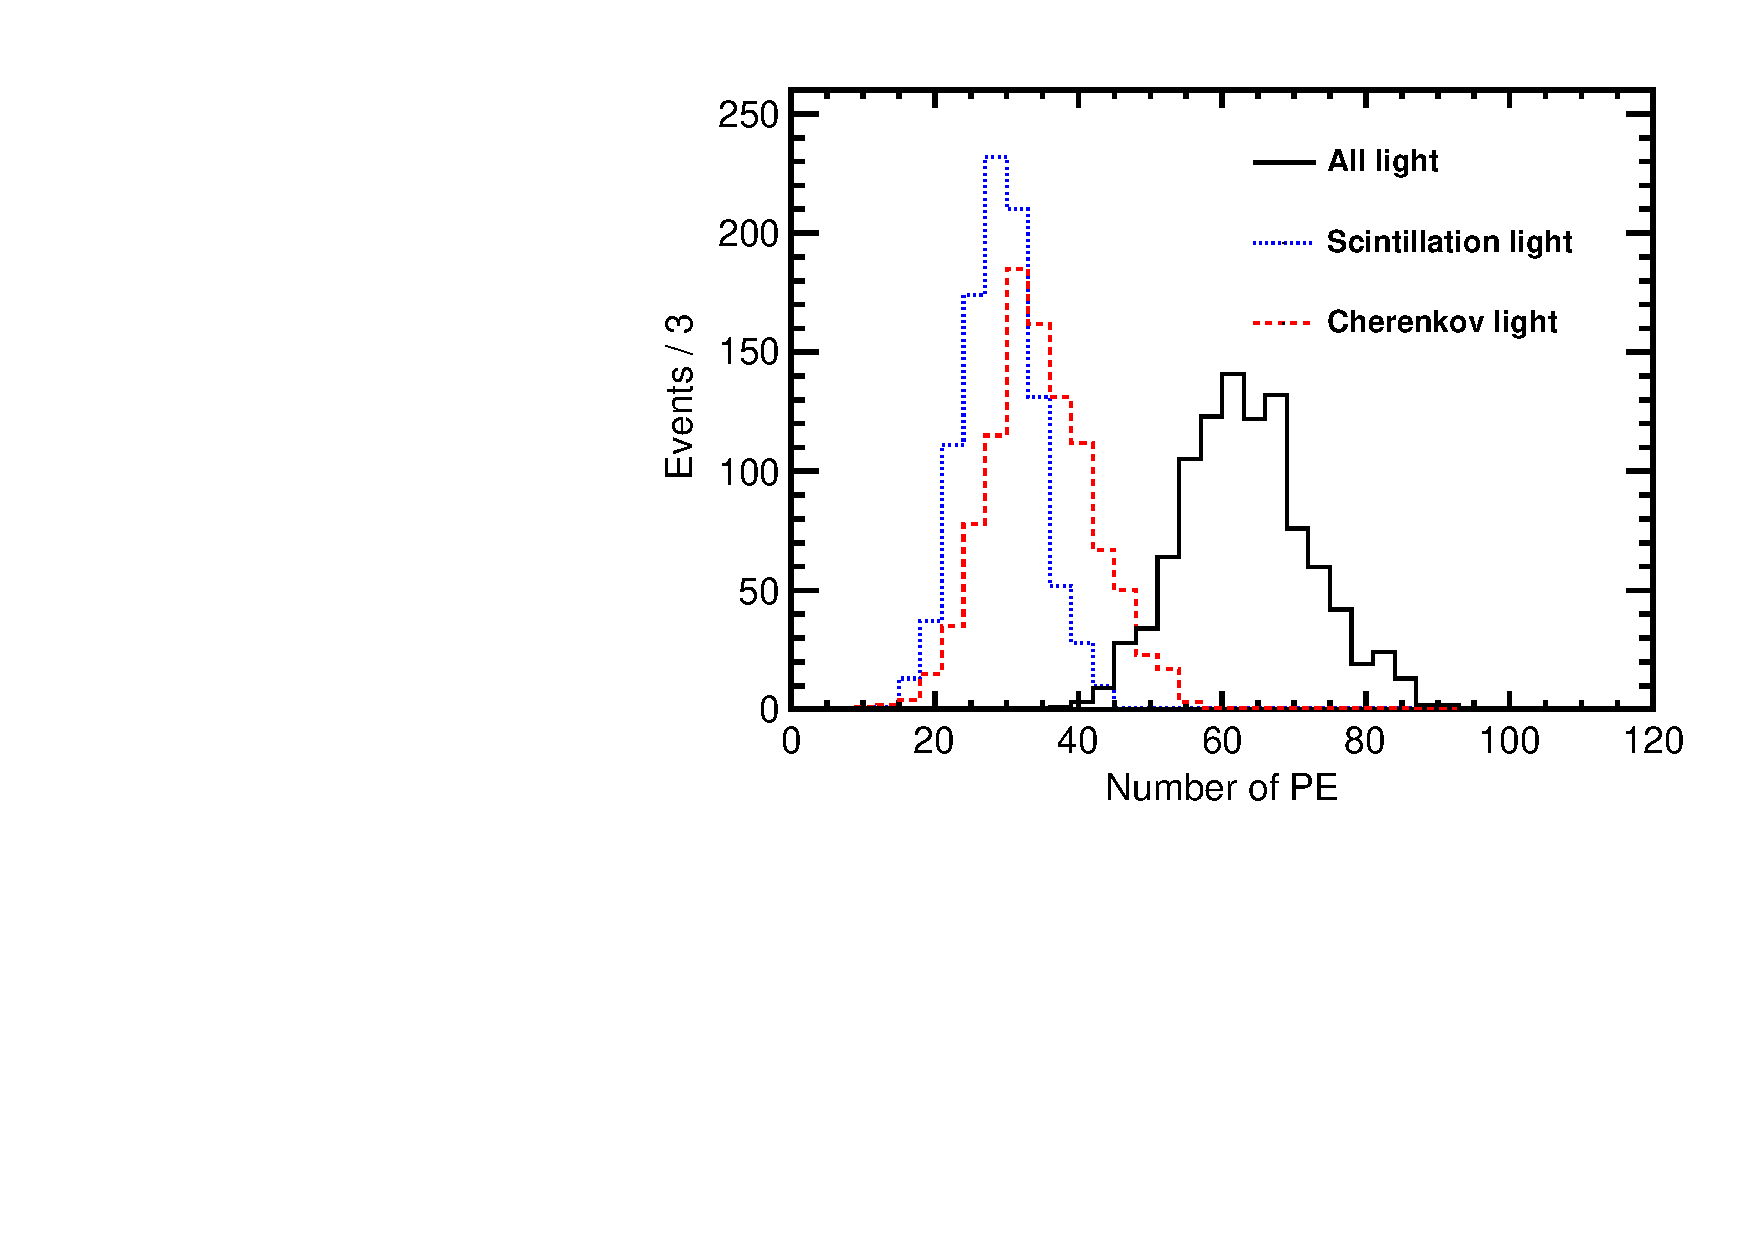
\includegraphics[width=0.45\textwidth]{hMomNPhot_Te130.pdf}
  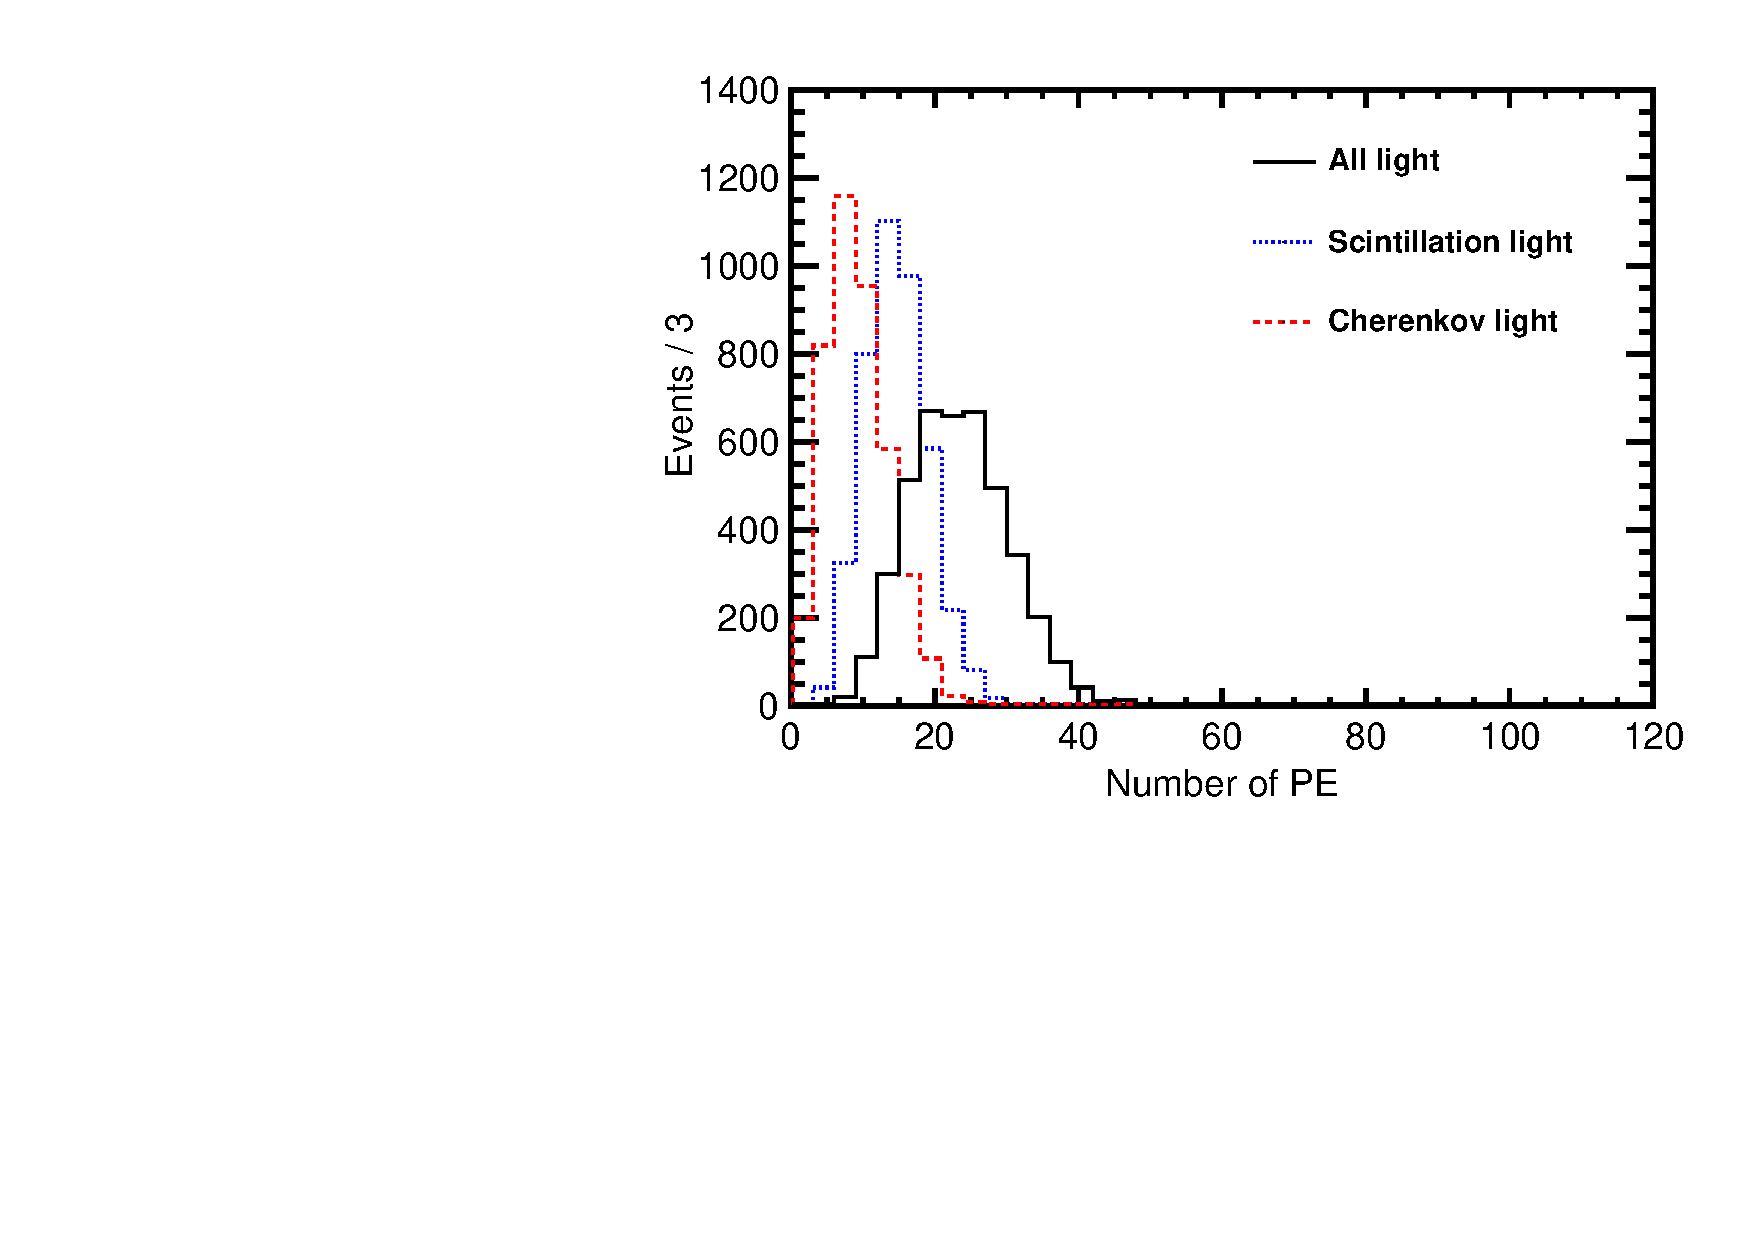
\includegraphics[width=0.45\textwidth]{hMomNPhot_C10.pdf}
  \caption{Number of PEs after 33.5~ns time cut applied to events simulated at the center
    of the detector. Cherenkov (\emph{dashed red line}), 
    scintillation (\emph{dotted blue line}), and total (\emph{solid black line}) PEs are
    compared separately for the simulation of 1000 $^{130}$Te 0{\nbb} decay (left panel)
    and of 4152 $^{10}$C (\emph{right panel}) events.} 
\label{fig:NPhotDist_C10}
\end{figure*}



\begin{figure*}[ht]
  \centering
  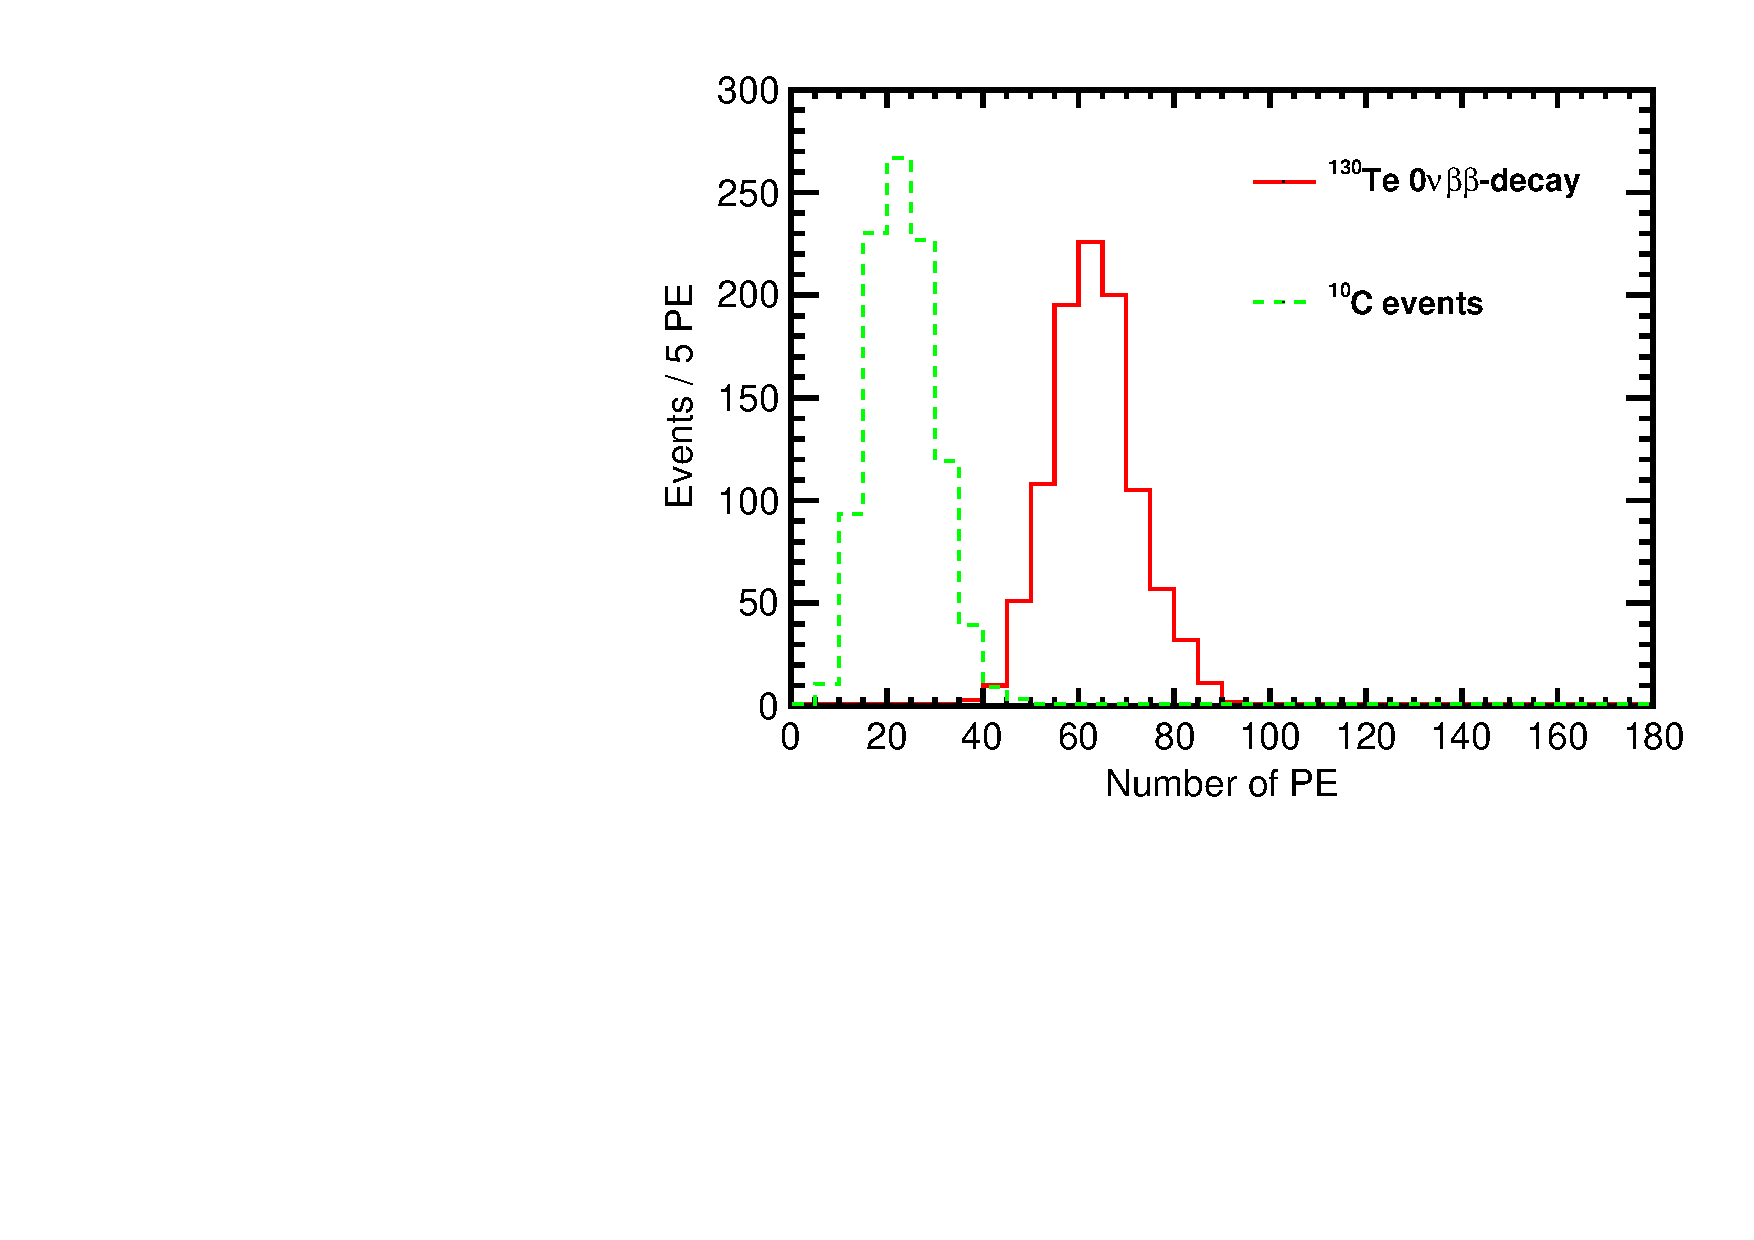
\includegraphics[width=0.95\textwidth]{hMomNPhot_Te130vsC10_allLight_VtxSmear0cm_VtxShiftX0cm_33p5ns_center.pdf}
  \caption{Total number of PEs in the early light sample. Comparison between $^{130}$Te 0{\nbb} decay 
    (solid red line) and $^{10}$C events (dashed greem line). Events are simulated at the center of the 
    detector. Perfect vertex reconstruction - true vertex position is used. Time cut of 
    33.5~ns on the photon arrival time is applied. Histograms are normalized to 1000 events.}
\label{fig:NPhot_compare_central}
\end{figure*}

Now we consider events with the primary vertex uniformly distributed within the fiducial volume of
R$<$3~m. In this case, the early light sample is defined as PEs with $\Delta T=T_{measured} -
T_{predicted}<$1~ns. Distributions of $\Delta T=T_{measured} - T_{predicted}$ for 
different assumptions on vertex resolution and corresponding total number of PEs in the early light
sample are shown in Figs.~\ref{fig:NPhot_compare_rndVtx_noSmear} - \ref{fig:NPhot_compare_rndVtx_Smear50cm}.

Figure~\ref{fig:NPhot_compare_rndVtx_noSmear} compares total number of PEs in the early light sample for 
events uniformly distributed within the fiducial volume and assuming perfect reconstruction of the primary 
vertex.

\begin{figure*}[ht]
  \centering
  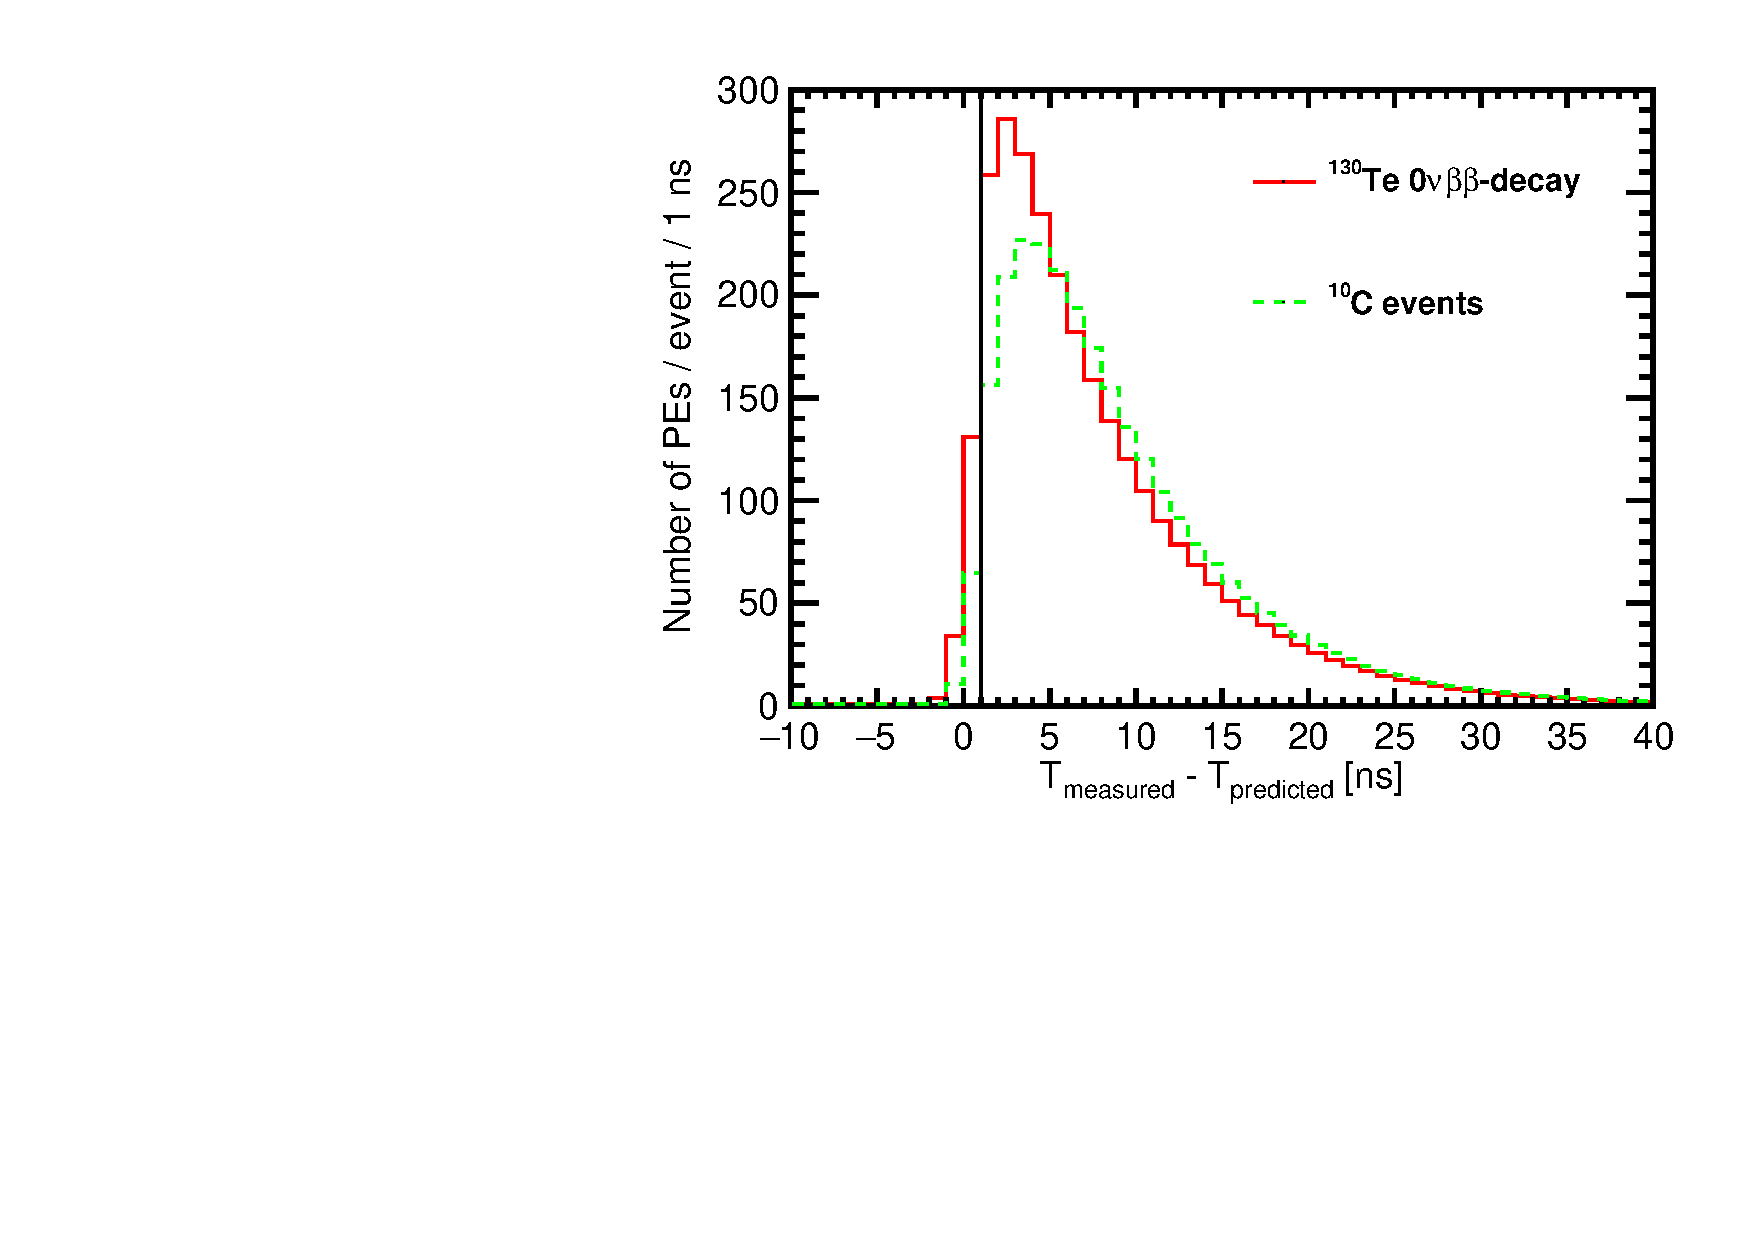
\includegraphics[width=0.45\textwidth]{hMomDT_Te130vsC10_allLight_VtxSmear0cm_VtxShiftX0cm_momDT1p0ns_rndVtx_3p0mSphere.pdf}
  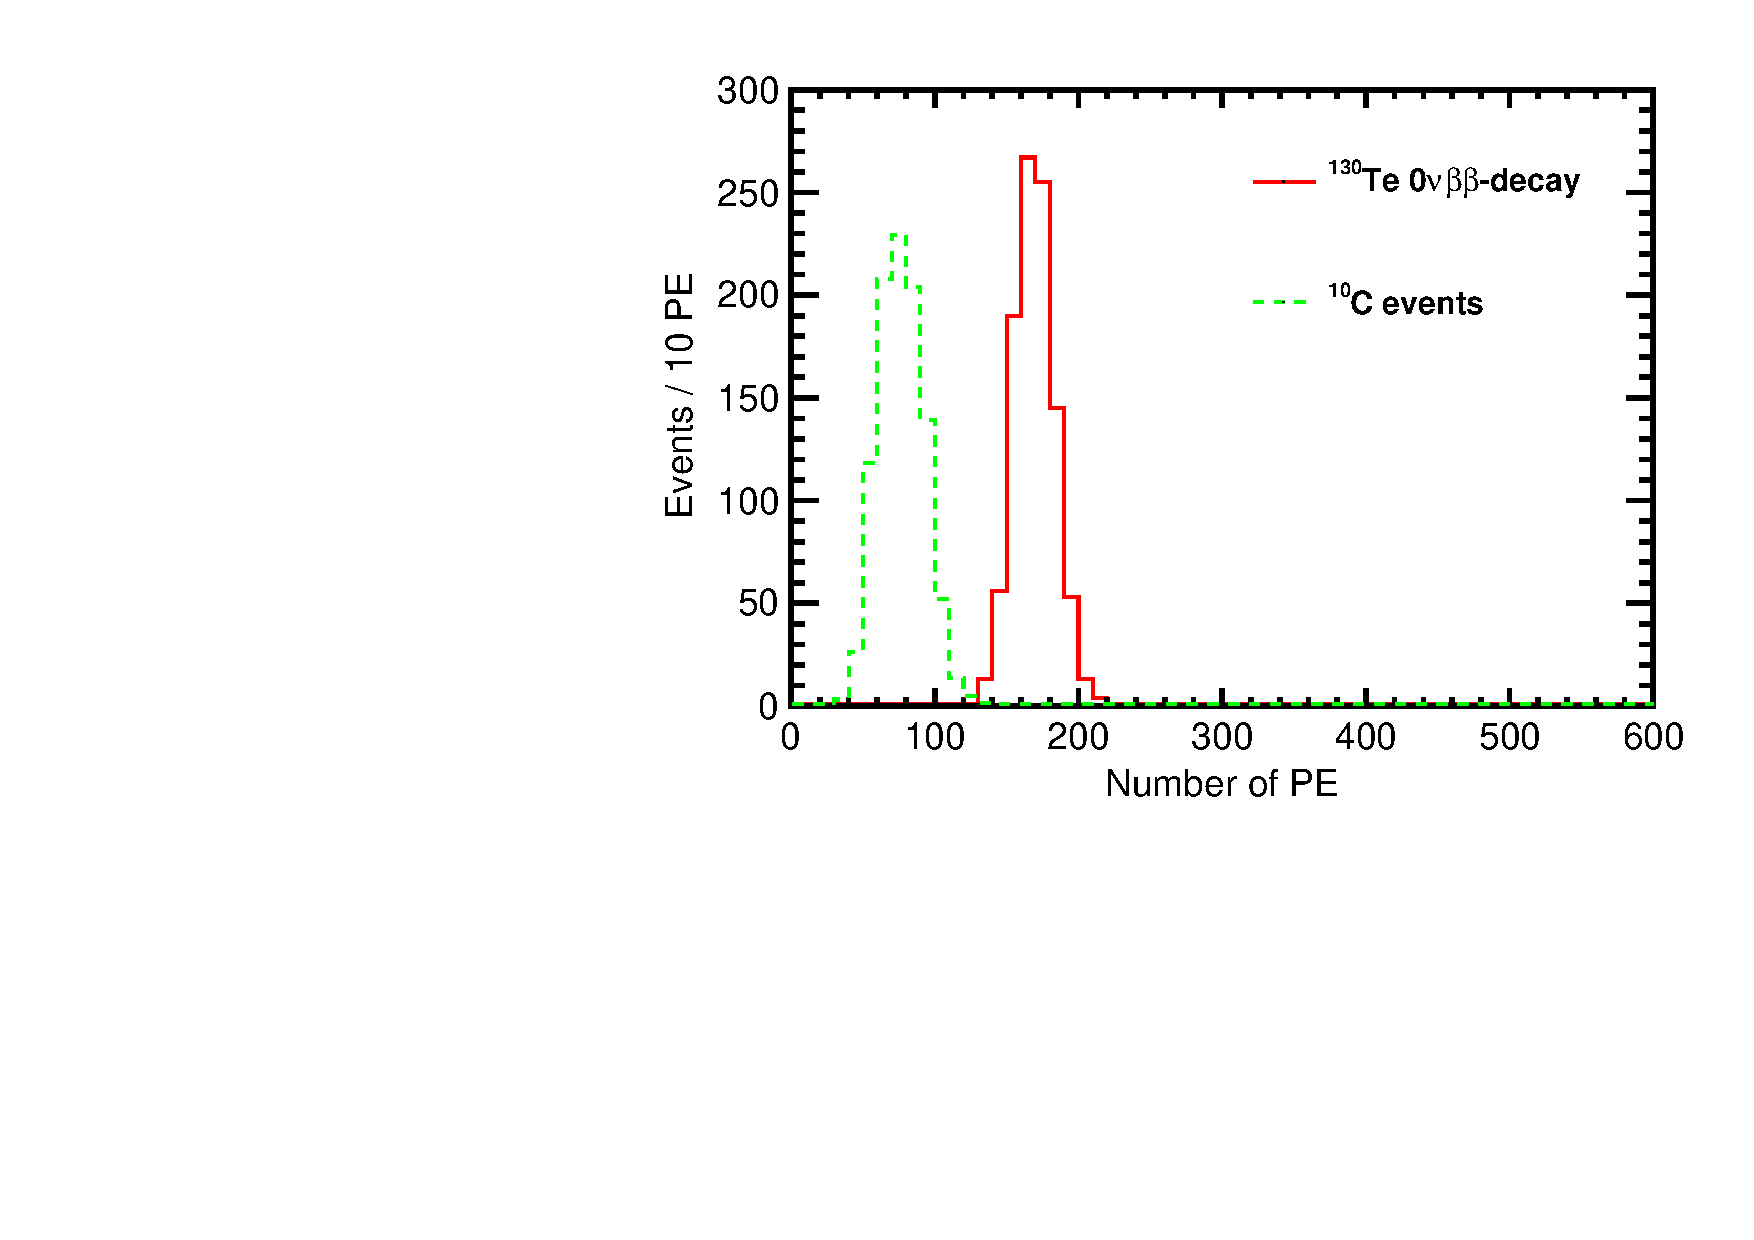
\includegraphics[width=0.45\textwidth]{hMomNPhot_Te130vsC10_allLight_VtxSmear0cm_VtxShiftX0cm_momDT1p0ns_rndVtx_3p0mSphere.pdf}
  \caption{(Left) Difference between measured PE arrival time and arrival time prediction based on 
	vertex location (T$^{predicted} = |r_{hit} - r_{vtx}|/v_{phot}$, where $v_phot = c/1.53$).
        $\vbb$-decay (black solid line) and $\Cten$ events (magenta dashed line) are compared. 
	Vertical line at 1~ns indicates cut for early light selection. 
        (Right) Total number of PEs in the early light sample. 
        $^{10}$C events with energy deposition in the $\pm$10\% energy range around Q-value are
	selected. Verticies are uniformly distributed within the fiducial volume, $R<3$~m.
        {\bf Perfect vertex reconstruction - true vertex position is used.}}
\label{fig:NPhot_compare_rndVtx_noSmear}
\end{figure*}


Figure~\ref{fig:NPhot_compare_rndVtx_Smear3cm} compares total number of PEs in the early light sample for 
events uniformly distributed within the fiducial volume and assuming $\sigma$=3~cm resolution on the primary 
vertex reconstruction. The effect of primary vertex reconstruction resolution is implemented as a smearing of 
the actual simulated vertex position, $R_{vtx}$, with the gaussian distribution, $G(R_{vtx},\sigma)$ 
which has sigma of $\sigma$ and mean of $R_{vtx}$. The resulting vertex position used in the calculation of the
predicted time $T_{predicted}$ is defined as $r_{vtx}$=$R_{vtx} + G(R_{vtx},\sigma)$.

\begin{figure*}[ht]
  \centering
  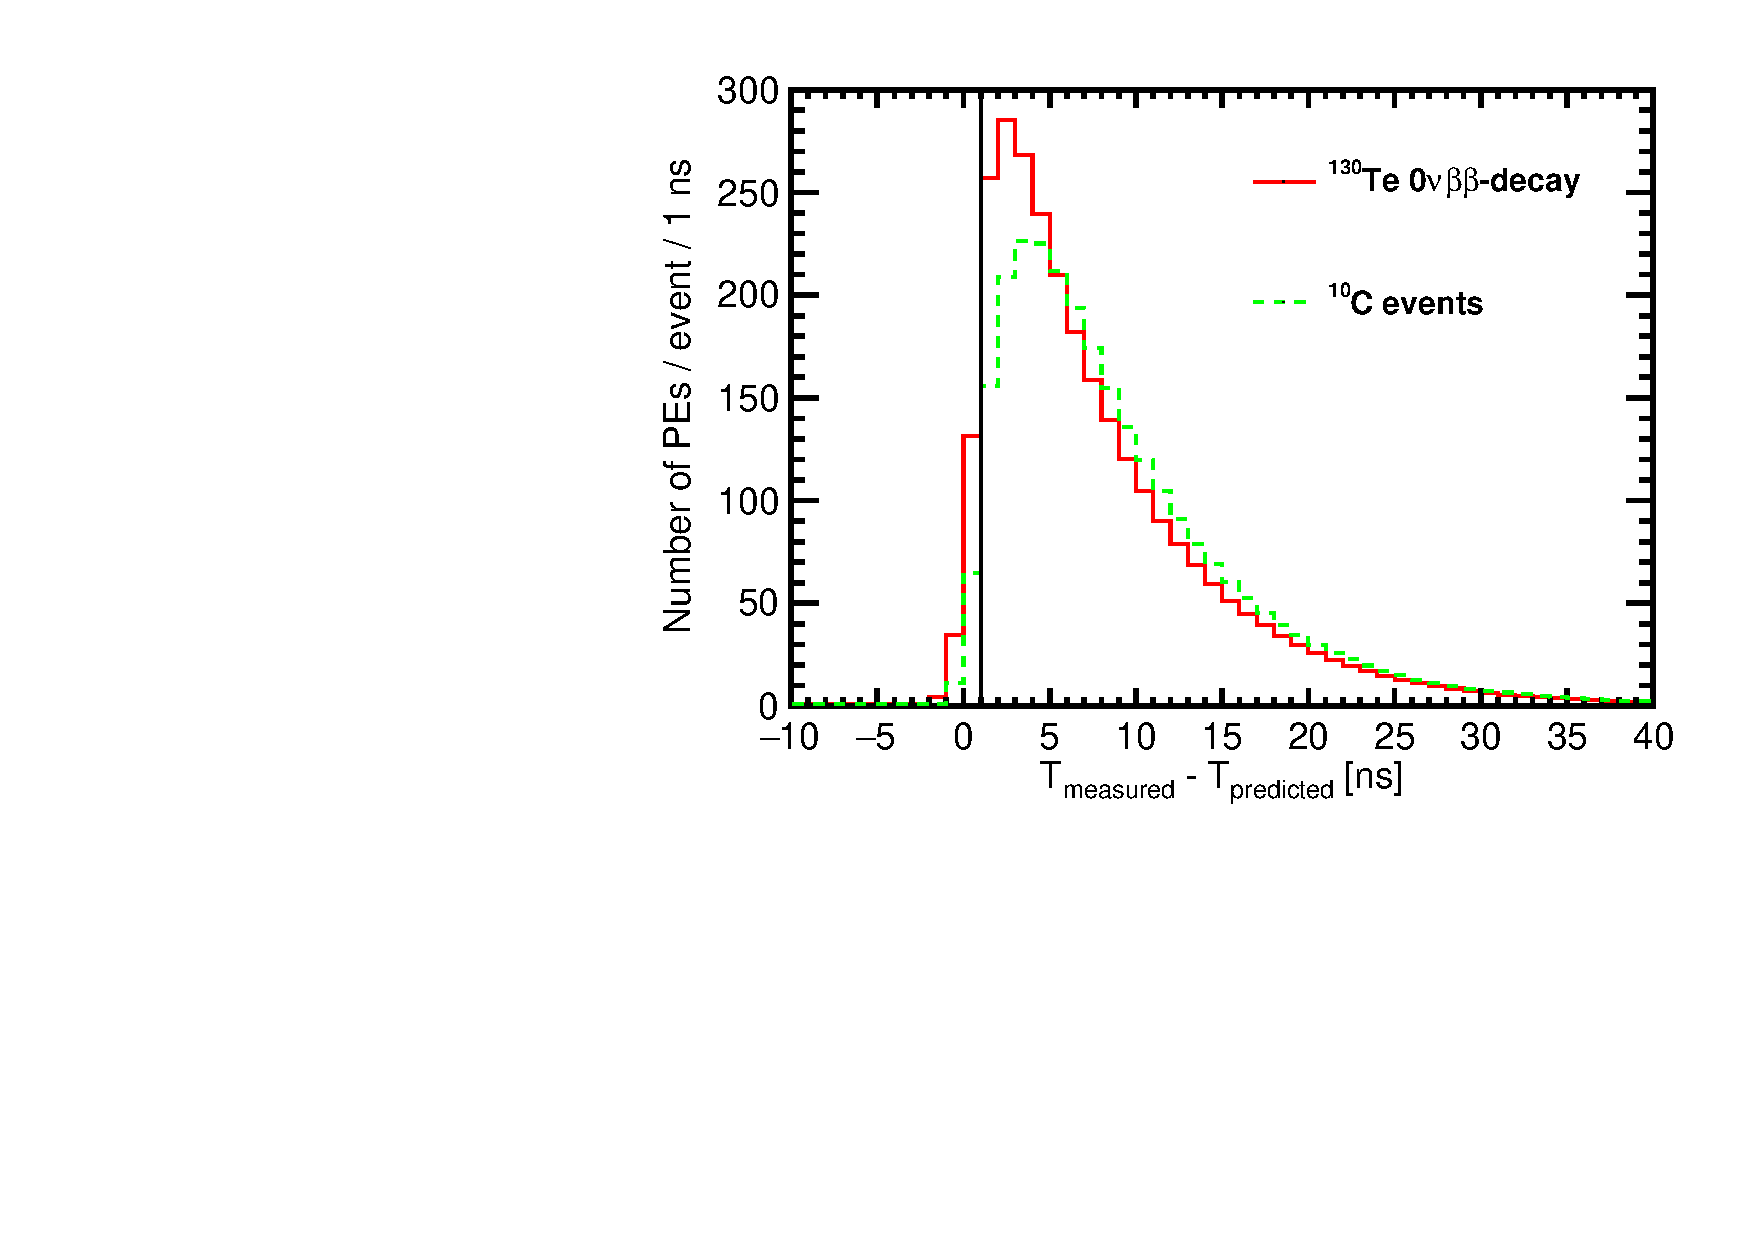
\includegraphics[width=0.45\textwidth]{hMomDT_Te130vsC10_allLight_VtxSmear3cm_VtxShiftX0cm_momDT1p0ns_rndVtx_3p0mSphere.pdf}
  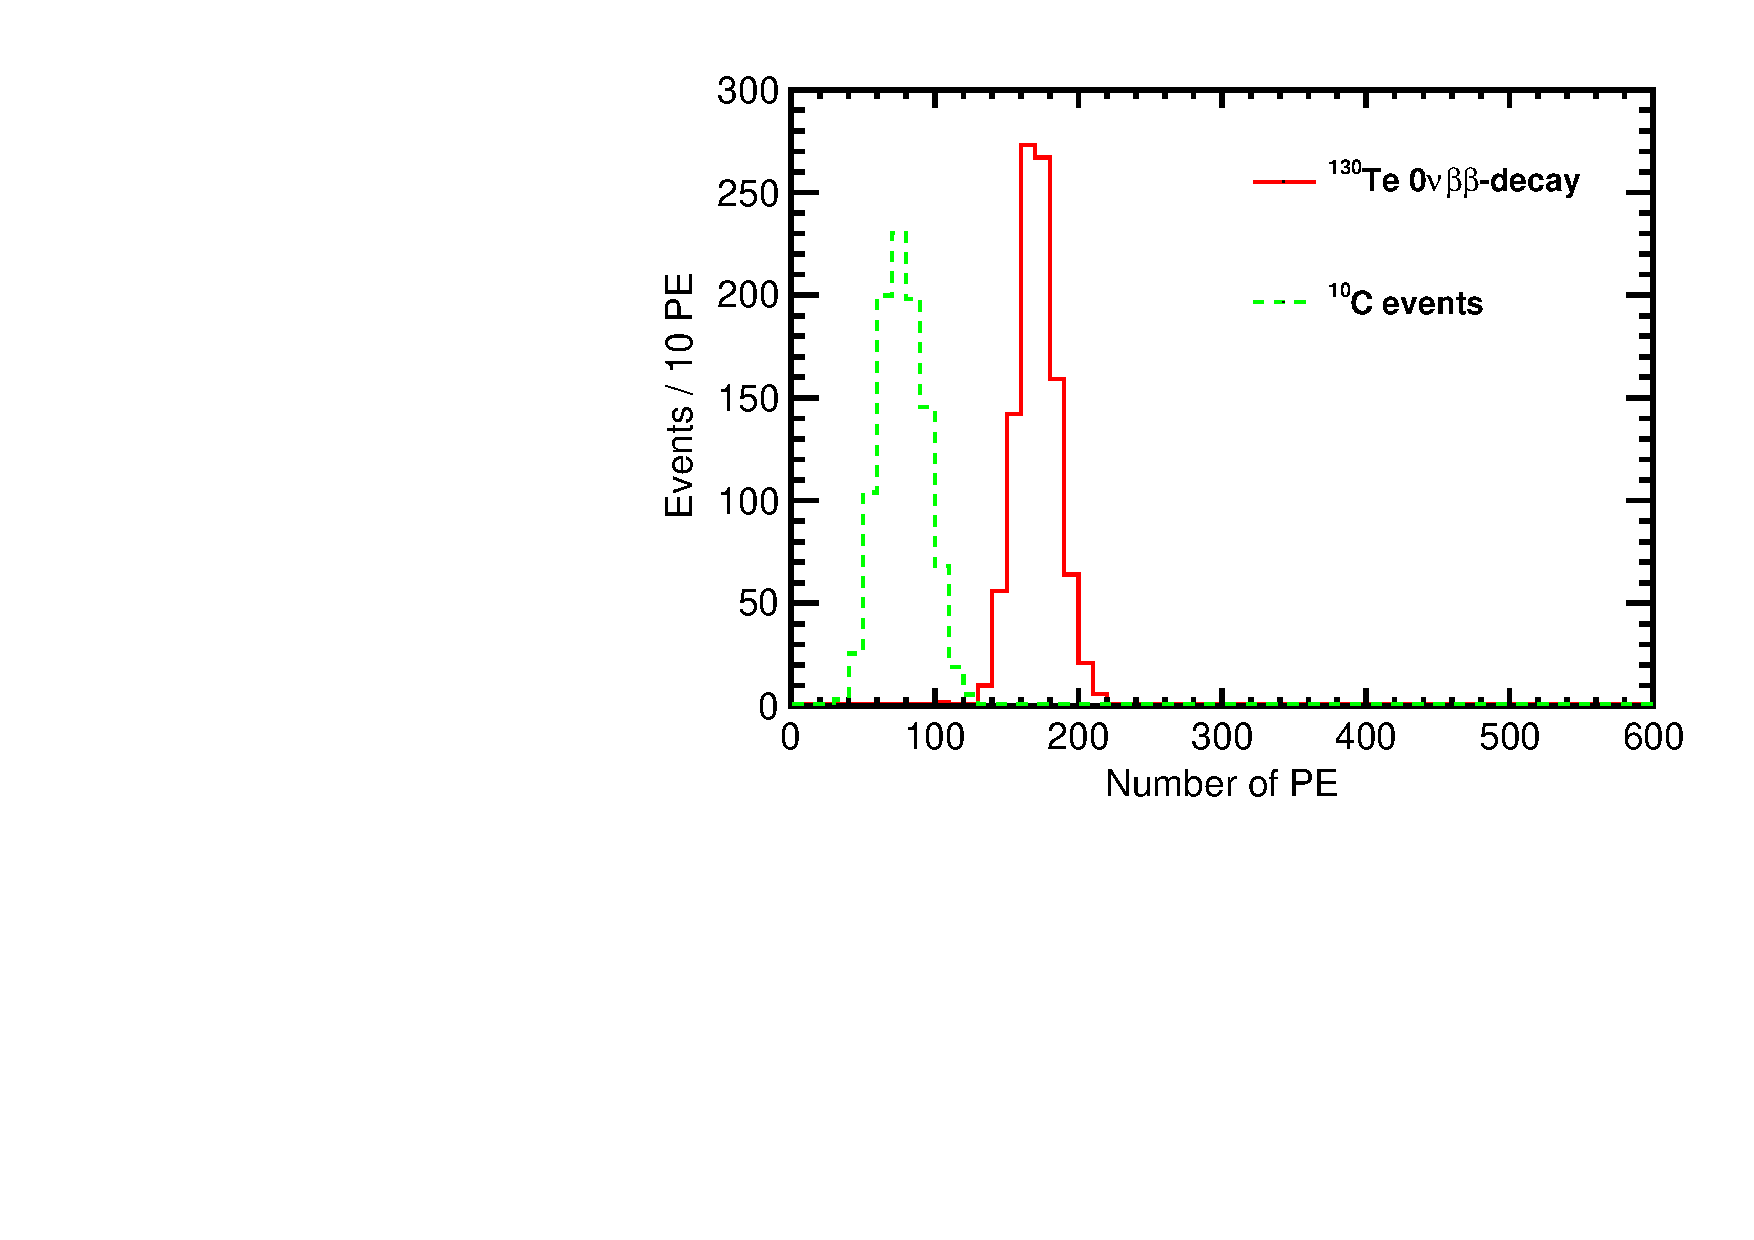
\includegraphics[width=0.45\textwidth]{hMomNPhot_Te130vsC10_allLight_VtxSmear3cm_VtxShiftX0cm_momDT1p0ns_rndVtx_3p0mSphere.pdf}
  \caption{(Left) Difference between measured PE arrival time and arrival time prediction based on
        vertex location (T$^{predicted} = |r_{hit} - r_{vtx}|/v_{phot}$, where $v_phot = c/1.53$).
        $\vbb$-decay (black solid line) and $\Cten$ events (magenta dashed line) are compared.
        Vertical line at 1~ns indicates cut for early light selection.
        (Right) Total number of PEs in the early light sample.
        $^{10}$C events with energy deposition in the $\pm$10\% energy range around Q-value are
        selected. Verticies are uniformly distributed within the fiducial volume, $R<3$~m.
        {\bf Vetrex is smeared with 3~cm resolution.}}
\label{fig:NPhot_compare_rndVtx_Smear3cm}
\end{figure*}


Figure~\ref{fig:NPhot_compare_rndVtx_Smear10cm} compares total number of PEs for events uniformly
distributed within the fiducial volume and reconstructed vertex smeared with 10~cm resolution.

\begin{figure*}[ht]
  \centering
  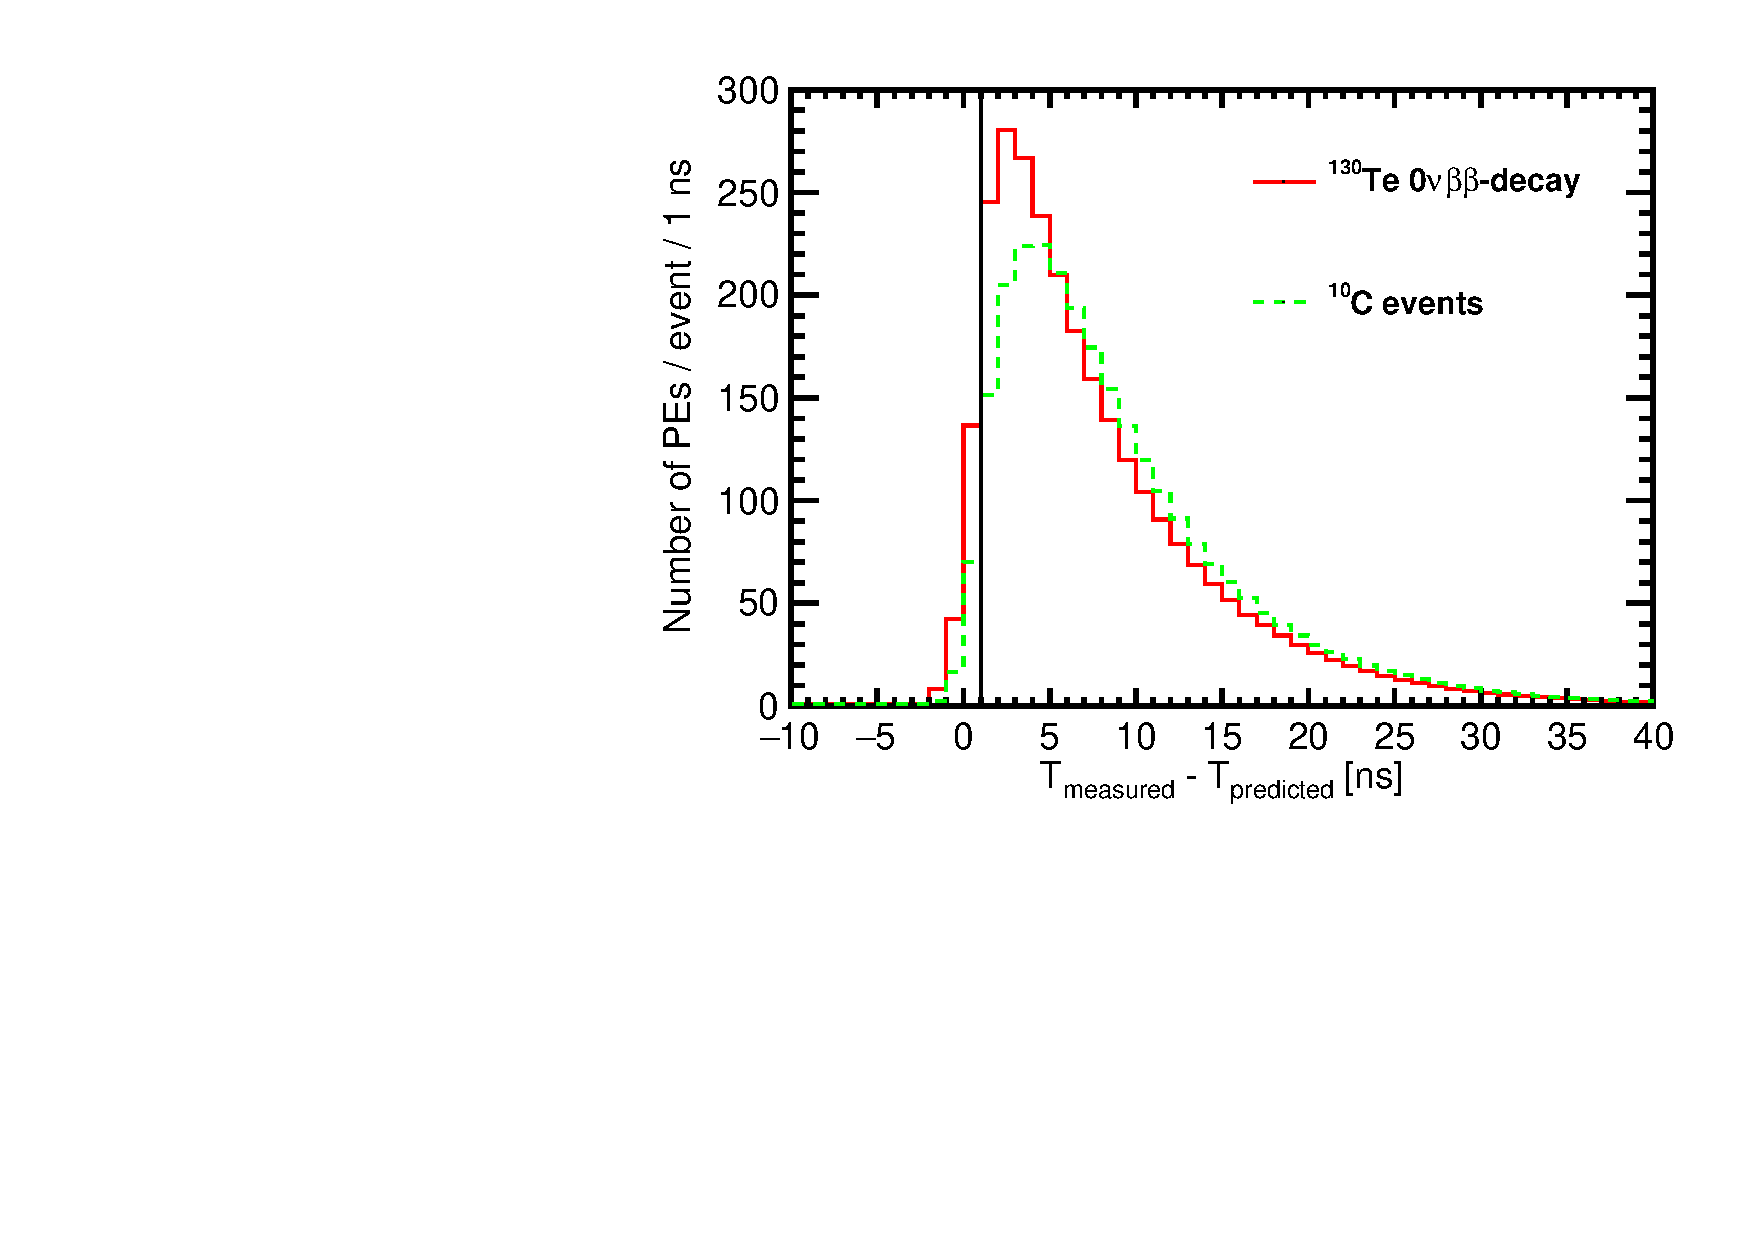
\includegraphics[width=0.45\textwidth]{hMomDT_Te130vsC10_allLight_VtxSmear10cm_VtxShiftX0cm_momDT1p0ns_rndVtx_3p0mSphere.pdf}
  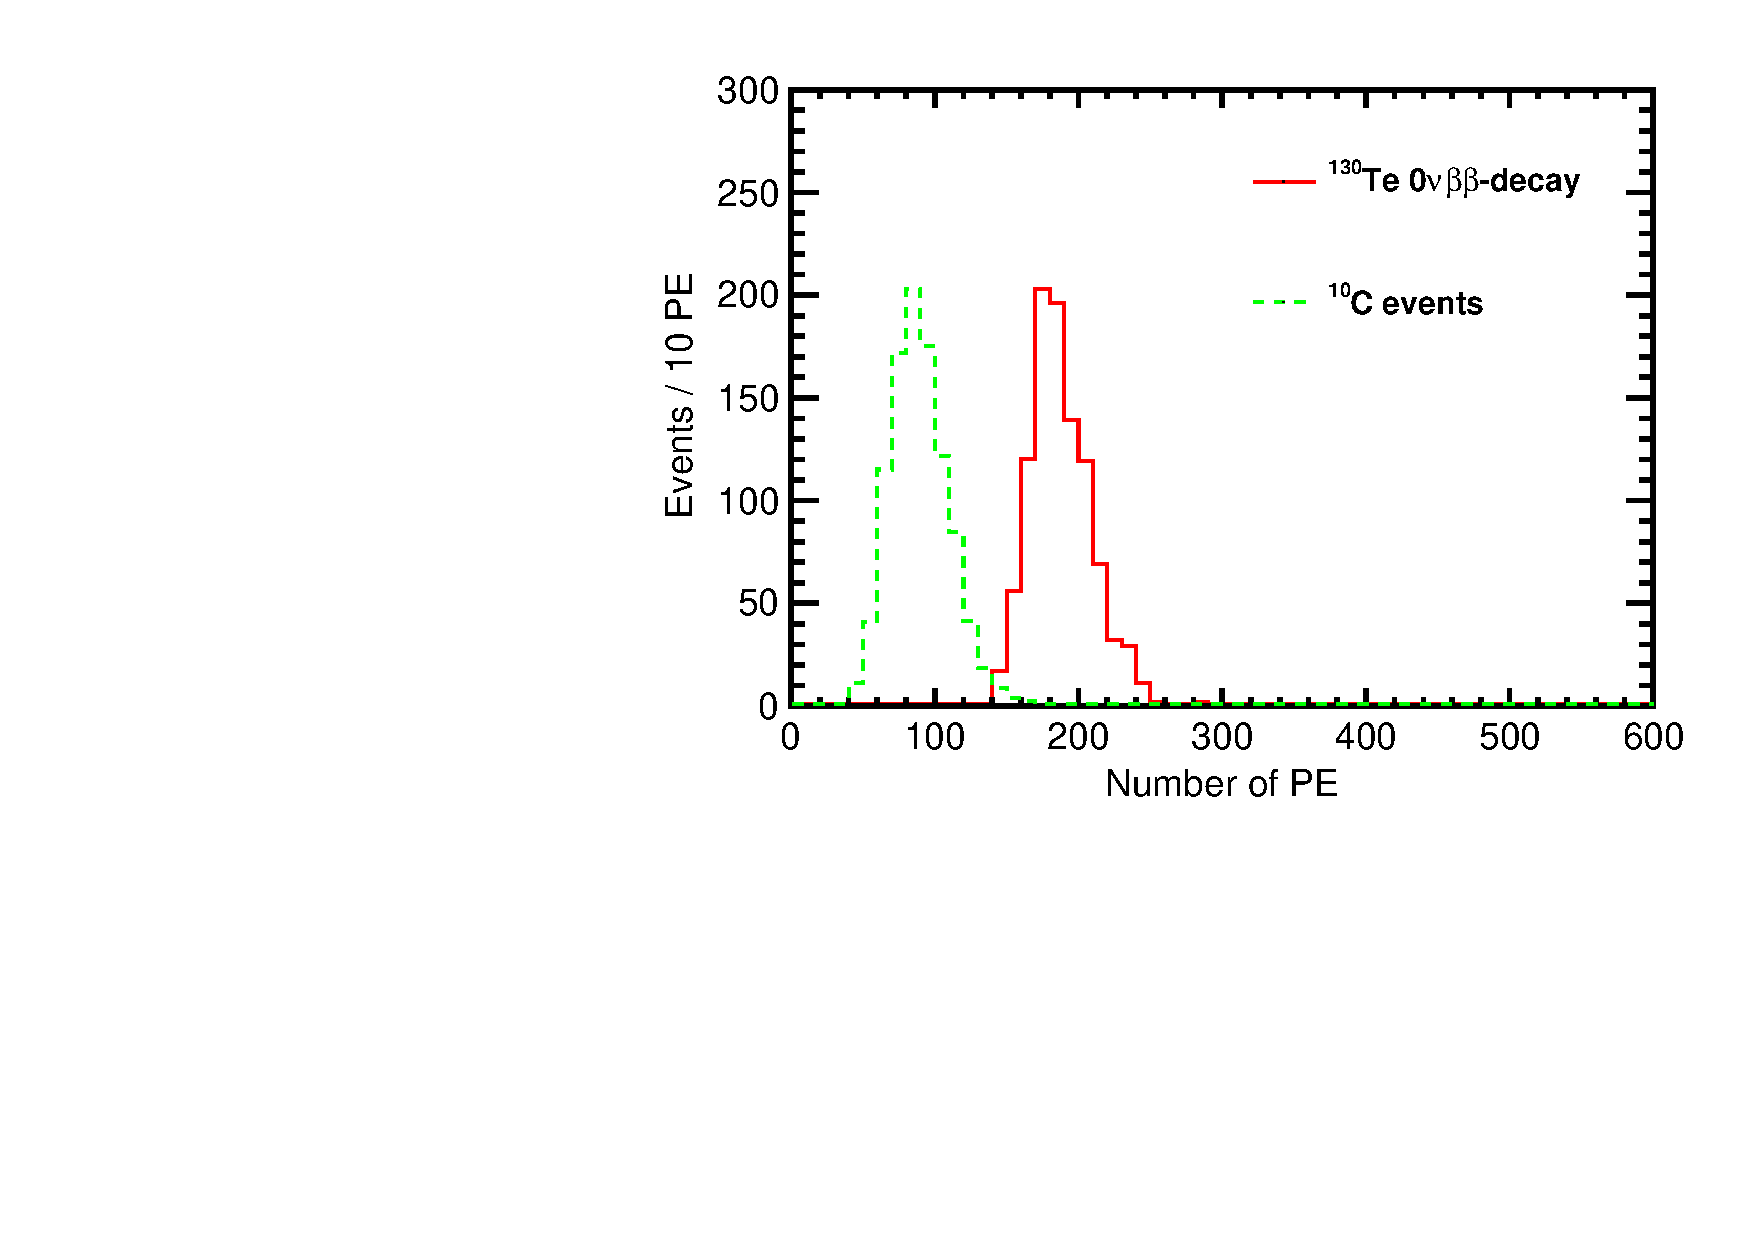
\includegraphics[width=0.45\textwidth]{hMomNPhot_Te130vsC10_allLight_VtxSmear10cm_VtxShiftX0cm_momDT1p0ns_rndVtx_3p0mSphere.pdf}
  \caption{(Left) Difference between measured PE arrival time and arrival time prediction based on
        vertex location (T$^{predicted} = |r_{hit} - r_{vtx}|/v_{phot}$, where $v_phot = c/1.53$).
        $\vbb$-decay (black solid line) and $\Cten$ events (magenta dashed line) are compared.
        Vertical line at 1~ns indicates cut for early light selection.
        (Right) Total number of PEs in the early light sample.
        $^{10}$C events with energy deposition in the $\pm$10\% energy range around Q-value are
        selected. Verticies are uniformly distributed within the fiducial volume, $R<3$~m.
        {\bf Vetrex is smeared with 10~cm resolution.}}
\label{fig:NPhot_compare_rndVtx_Smear10cm}
\end{figure*}



Figure~\ref{fig:NPhot_compare_rndVtx_Smear30cm} compares total number of PEs for events uniformly
distributed within the fiducial volume and reconstructed vertex smeared with 30~cm resolution.

\begin{figure*}[ht]
  \centering
  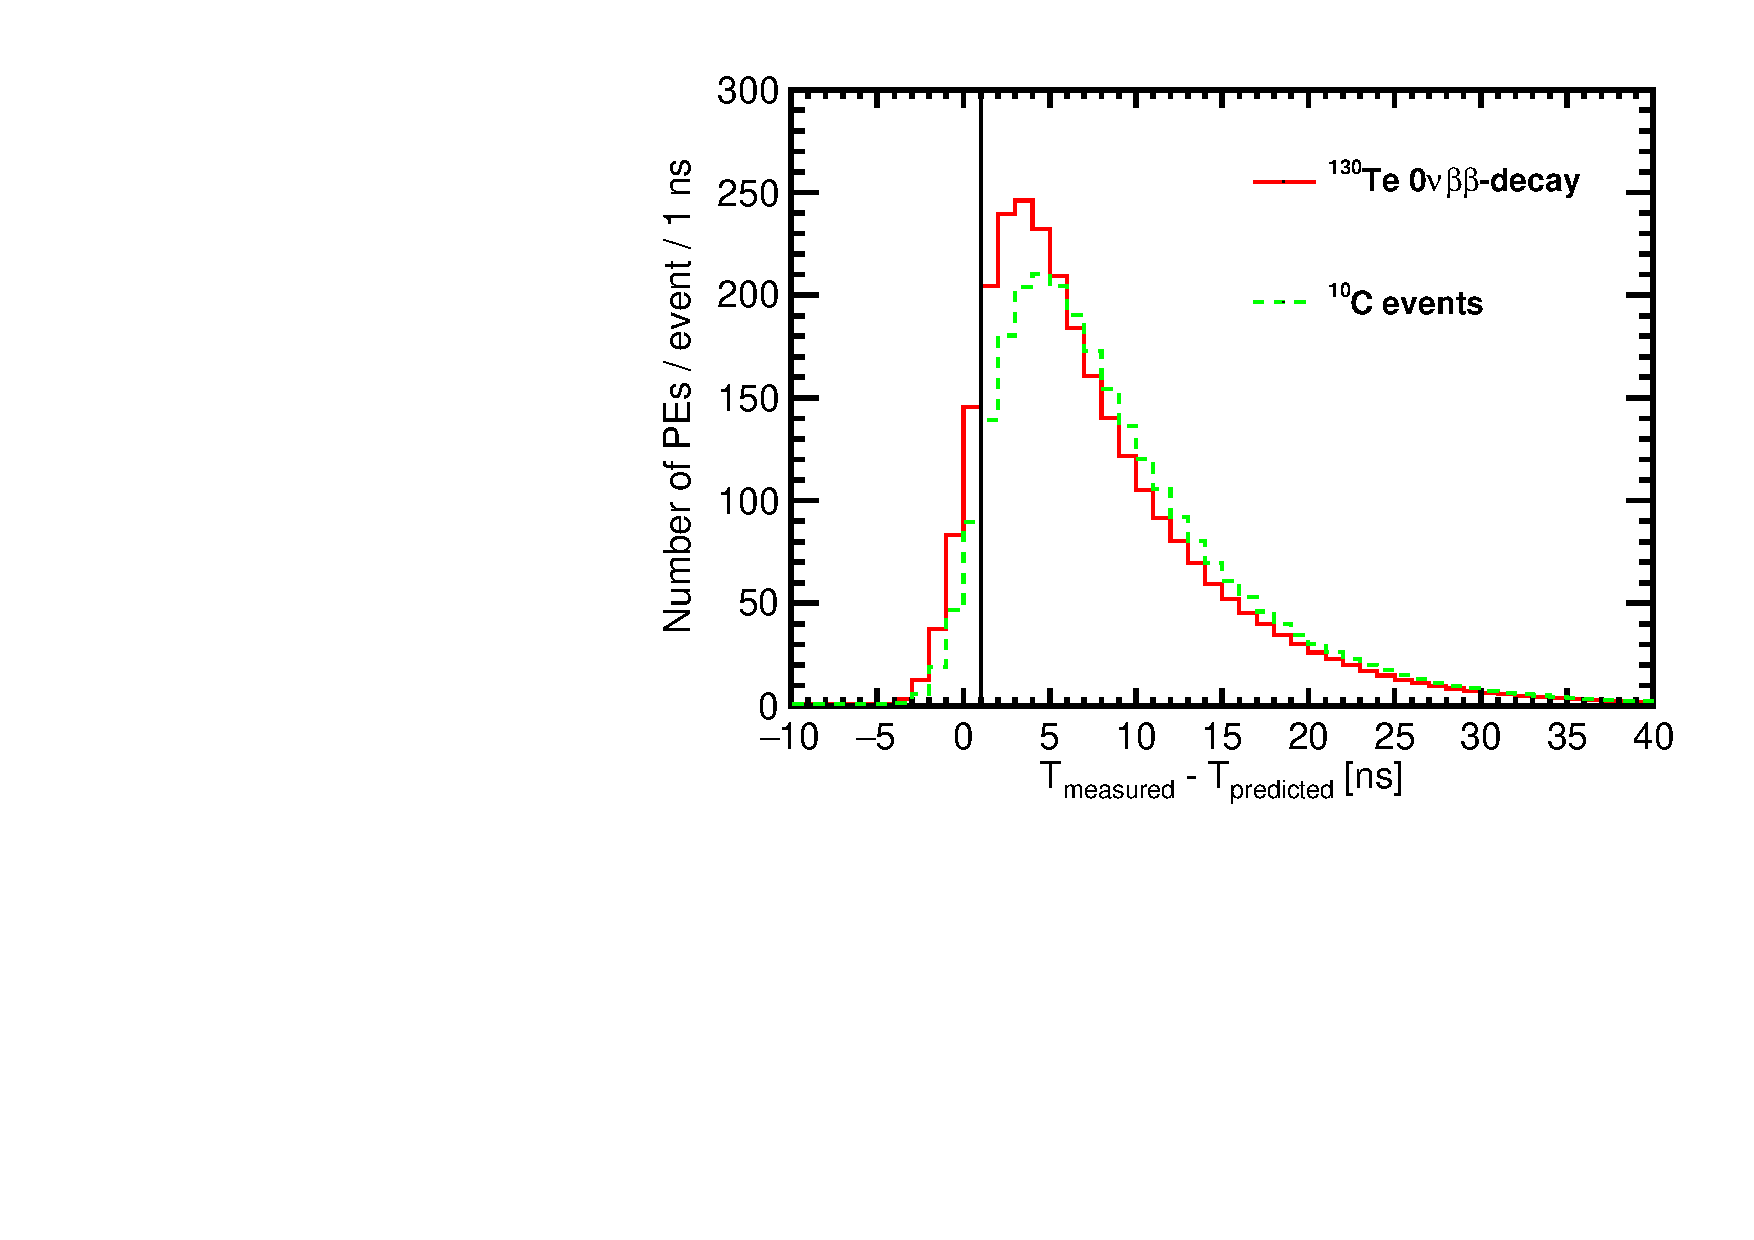
\includegraphics[width=0.45\textwidth]{hMomDT_Te130vsC10_allLight_VtxSmear30cm_VtxShiftX0cm_momDT1p0ns_rndVtx_3p0mSphere.pdf}
  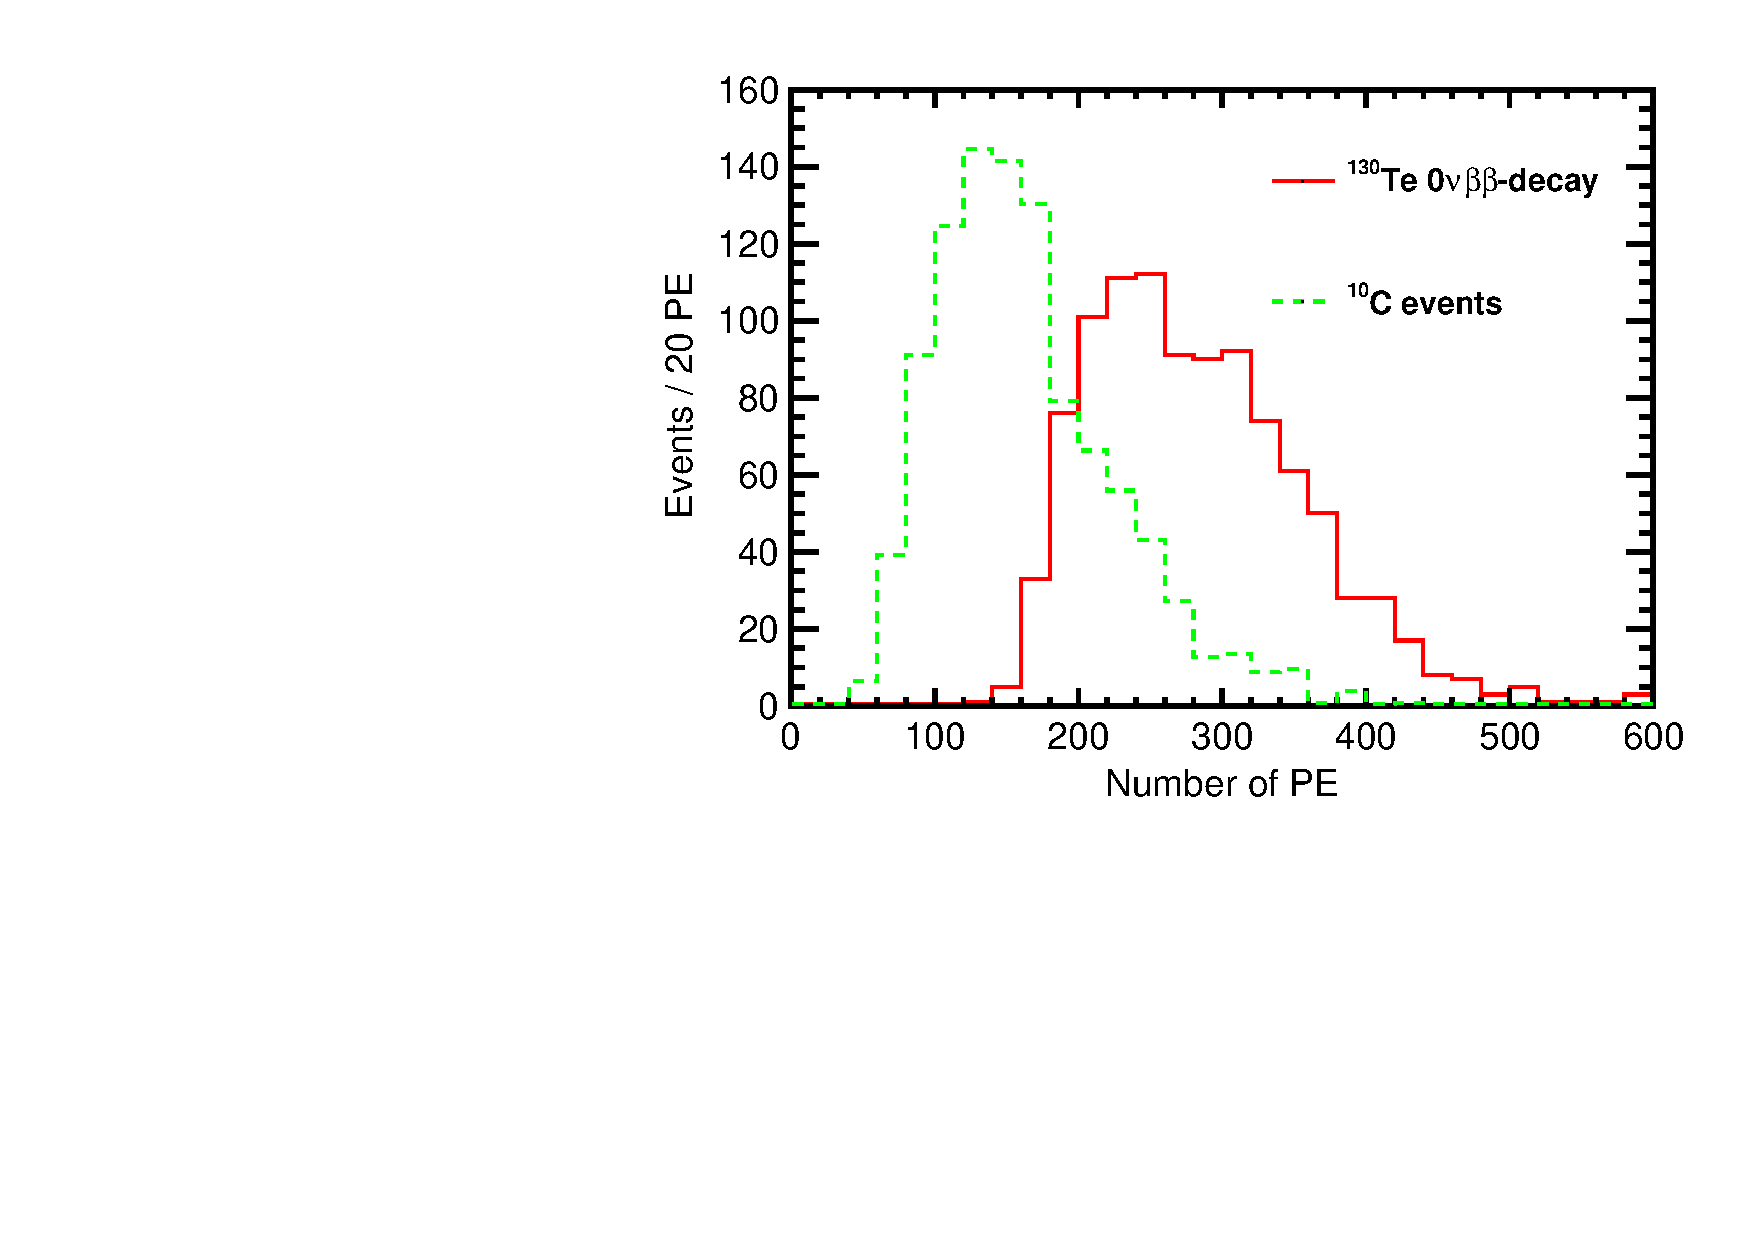
\includegraphics[width=0.45\textwidth]{hMomNPhot_Te130vsC10_allLight_VtxSmear30cm_VtxShiftX0cm_momDT1p0ns_rndVtx_3p0mSphere.pdf}
  \caption{(Left) Difference between measured PE arrival time and arrival time prediction based on
        vertex location (T$^{predicted} = |r_{hit} - r_{vtx}|/v_{phot}$, where $v_phot = c/1.53$).
        $\vbb$-decay (black solid line) and $\Cten$ events (magenta dashed line) are compared.
        Vertical line at 1~ns indicates cut for early light selection.
        (Right) Total number of PEs in the early light sample.
        $^{10}$C events with energy deposition in the $\pm$10\% energy range around Q-value. are
        selected. Verticies are uniformly distributed within the fiducial volume, $R<3$~m.
        {\bf Vetrex is smeared with 30~cm resolution.}}
\label{fig:NPhot_compare_rndVtx_Smear30cm}
\end{figure*}


Figure~\ref{fig:NPhot_compare_rndVtx_Smear50cm} compares total number of PEs for events uniformly
distributed within the fiducial volume and reconstructed vertex smeared with 50~cm resolution.

\begin{figure*}[ht]
  \centering
  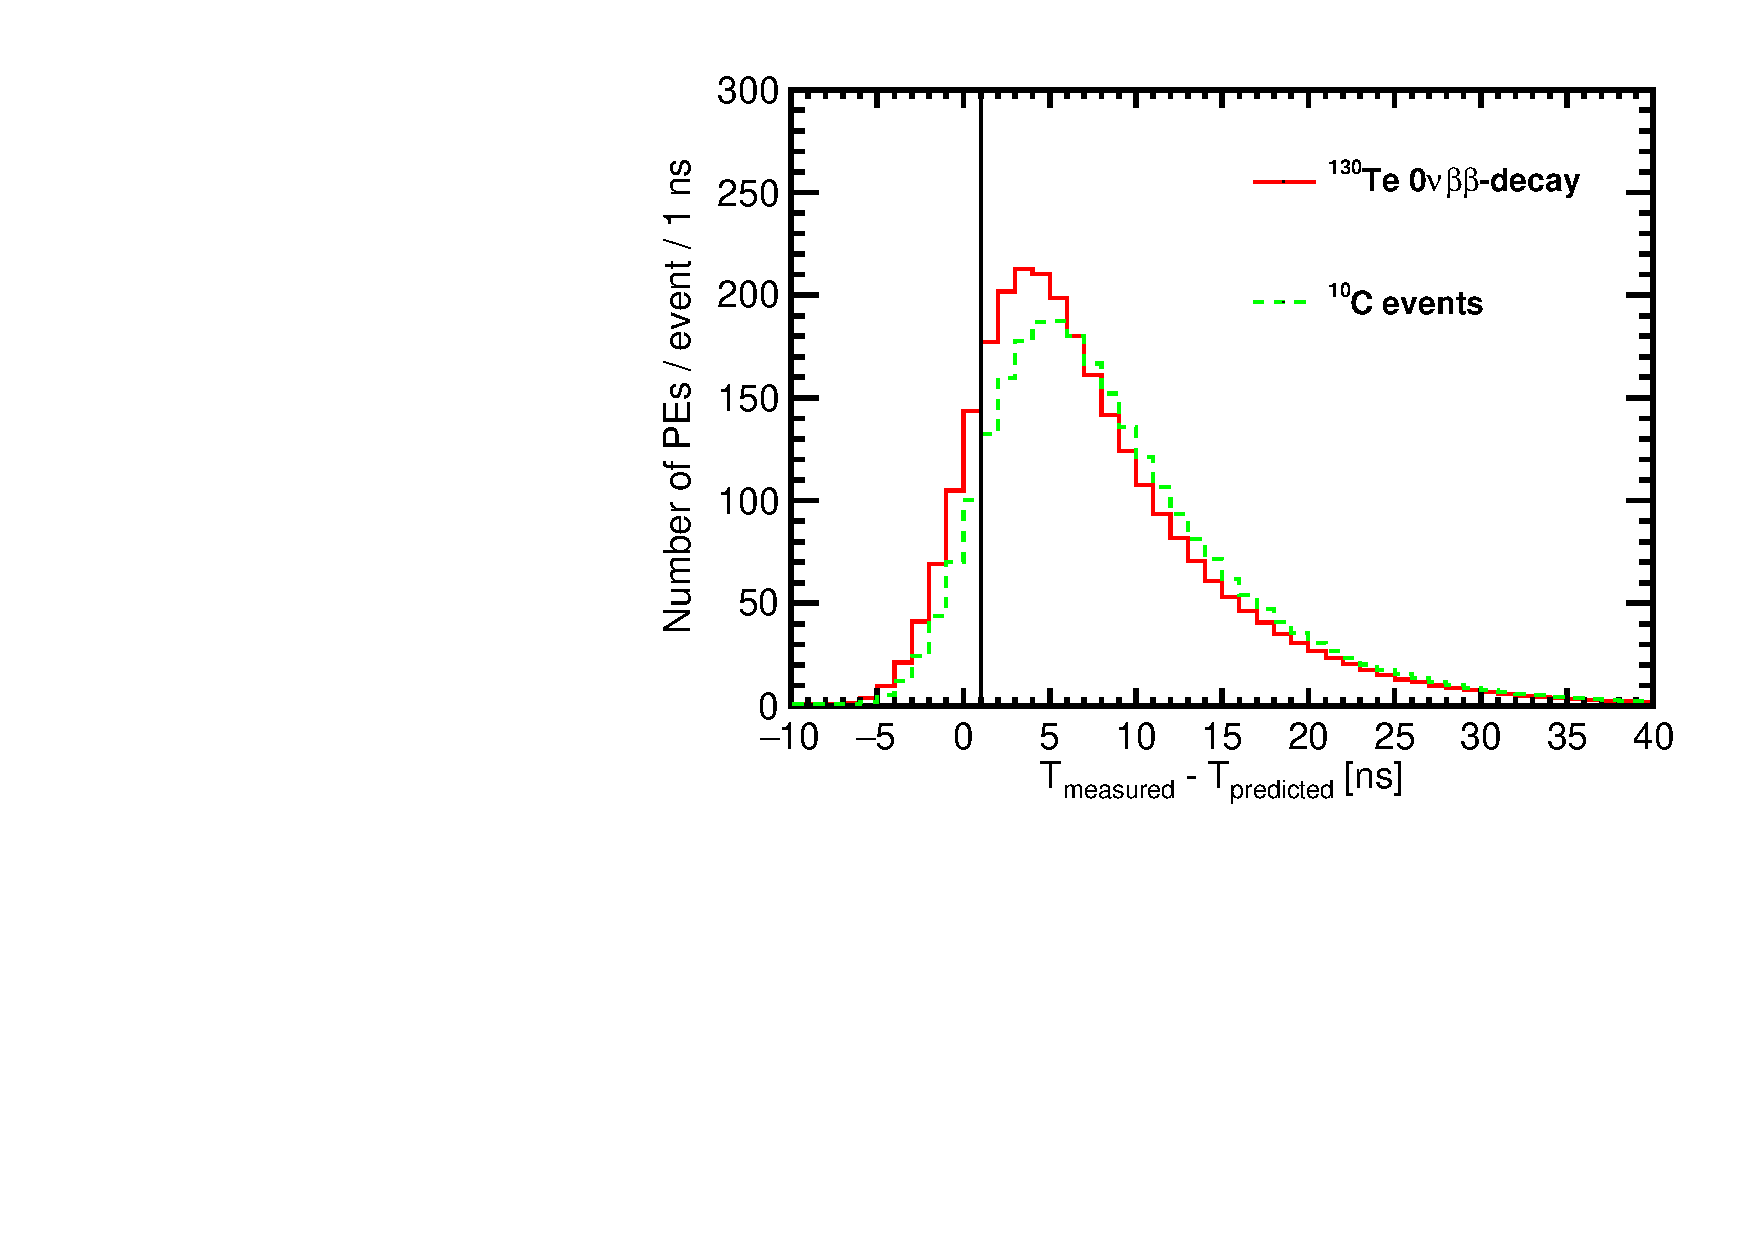
\includegraphics[width=0.45\textwidth]{hMomDT_Te130vsC10_allLight_VtxSmear50cm_VtxShiftX0cm_momDT1p0ns_rndVtx_3p0mSphere.pdf}
  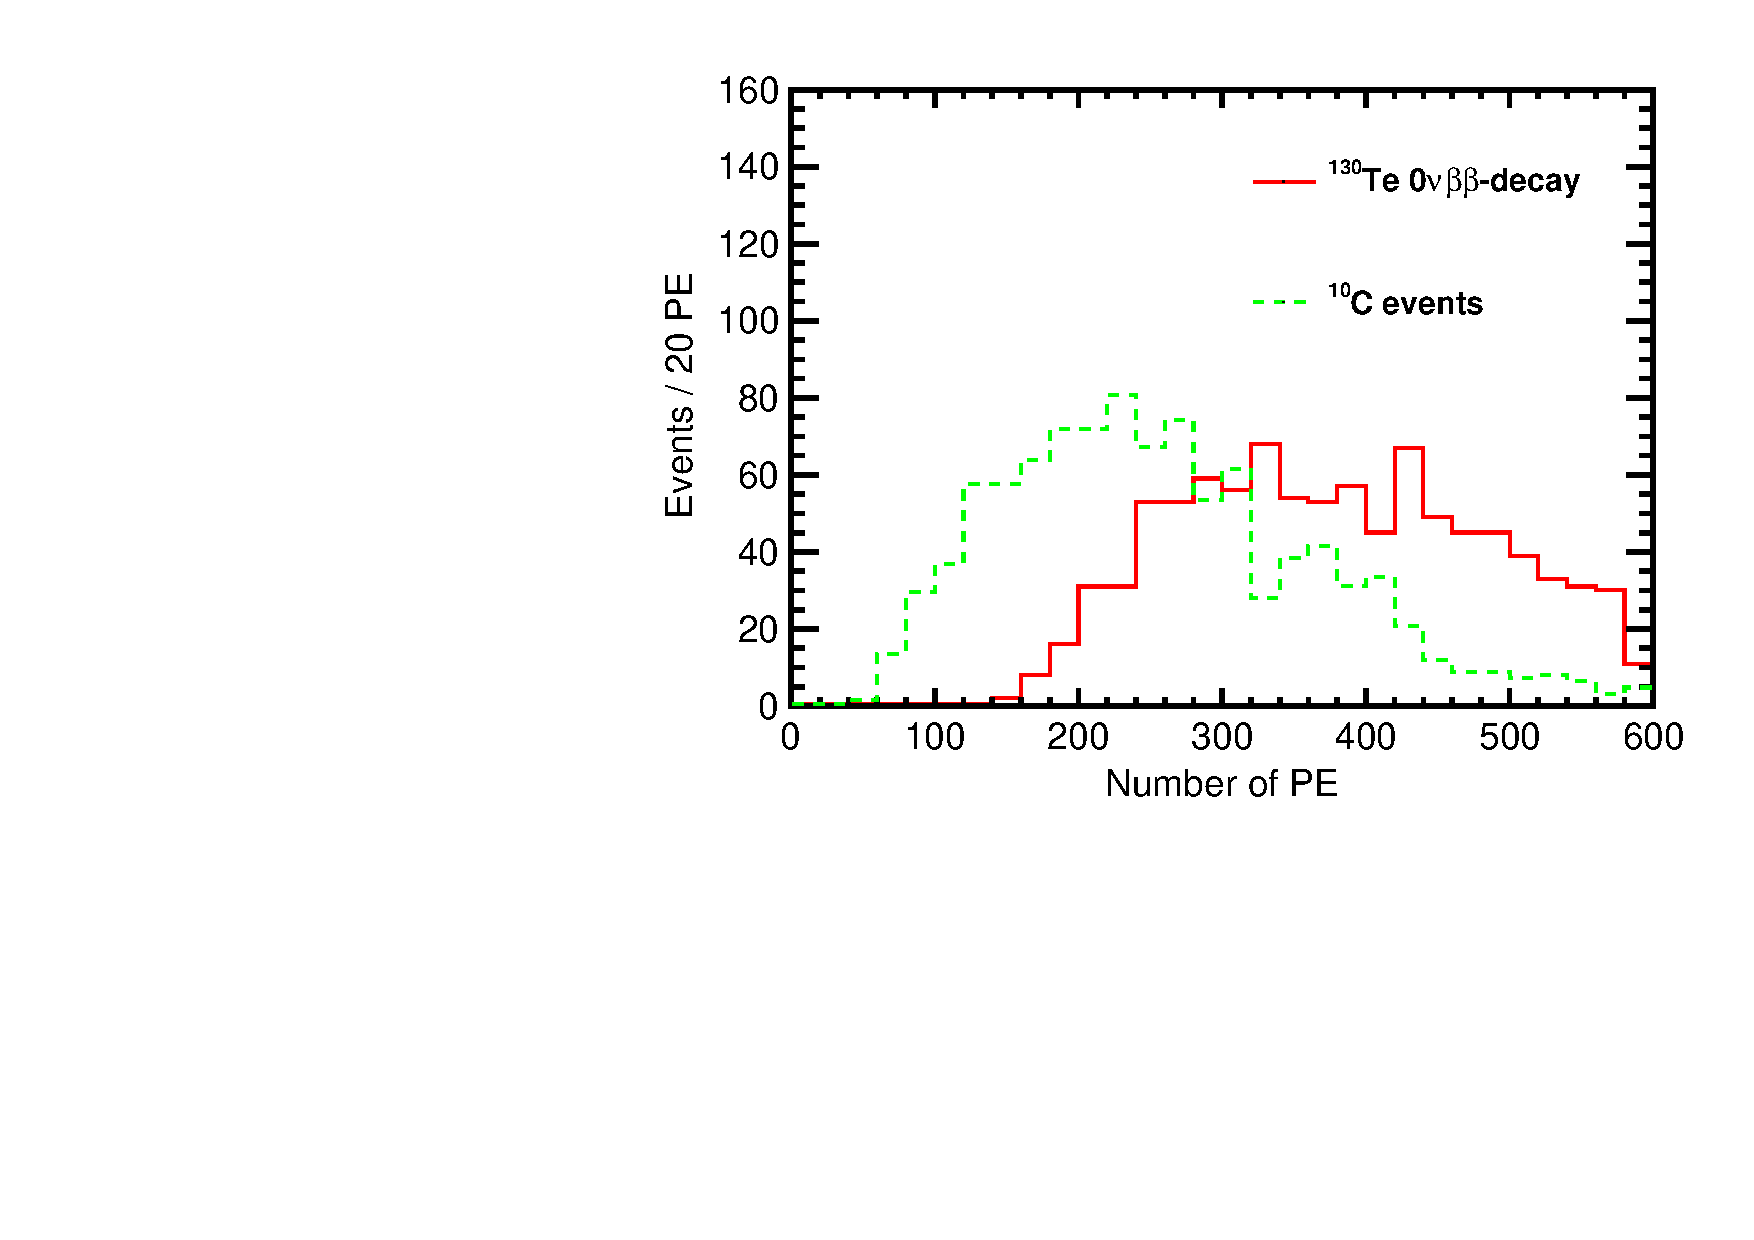
\includegraphics[width=0.45\textwidth]{hMomNPhot_Te130vsC10_allLight_VtxSmear50cm_VtxShiftX0cm_momDT1p0ns_rndVtx_3p0mSphere.pdf}
  \caption{(Left) Difference between measured PE arrival time and arrival time prediction based on
        vertex location (T$^{predicted} = |r_{hit} - r_{vtx}|/v_{phot}$, where $v_phot = c/1.53$).
        $\vbb$-decay (black solid line) and $\Cten$ events (magenta dashed line) are compared.
        Vertical line at 1~ns indicates cut for early light selection.
        (Right) Total number of PEs in the early light sample.
        $^{10}$C events with energy deposition in the $\pm$10\% energy range around Q-value are
        selected. Verticies are uniformly distributed within the fiducial volume, $R<3$~m.
        {\bf Vetrex is smeared with 50~cm resolution.}}
\label{fig:NPhot_compare_rndVtx_Smear50cm}
\end{figure*}



% !!!!!!!!!!!!	Commented text begins	!!!!!!!!!!!!!!!!!!!!!
\begin{comment}
\newpage

\section{0{\nbb} decay vs $^{10}$C background}

Other common backgrounds to 0{\nbb} decay search include radioactive
decays of nuclei that are excited by cosmic muons and produced through the decays of Th and U
naturally present in the materials. In liquid scintillator detectors,
most of events from Th and U decays occur in the materials of
the scintillator enclosure. Typically, they enter the fiducial volume
as 2.6~MeV gammas. These gammas pass into the fiducial volume either because they showered too late or have
mis-reconstructed vertex. Both effects depend on details of a
particular experiment and in this paper we make no attempt
to introduce a topology reconstruction for the backgrounds coming from
Th and U lines. Cosmic induced backgrounds, to the contrary, are more
generic and originate inside the fiducial volume. In this section we
discuss event topology of $^{10}$C events that are most relevant in the
energy of 2-3~MeV.

Typical energy deposition by $^{10}$C events is shown in
Fig.~\ref{fig:Edep_C10}. We propose to use spherical harmonics
analysis to separate 0{\nbb} decay events from $^{10}$C events that
within energy resolution overlap with the 0{\nbb} decay Q-value.

\begin{figure}[h]
  \centering
  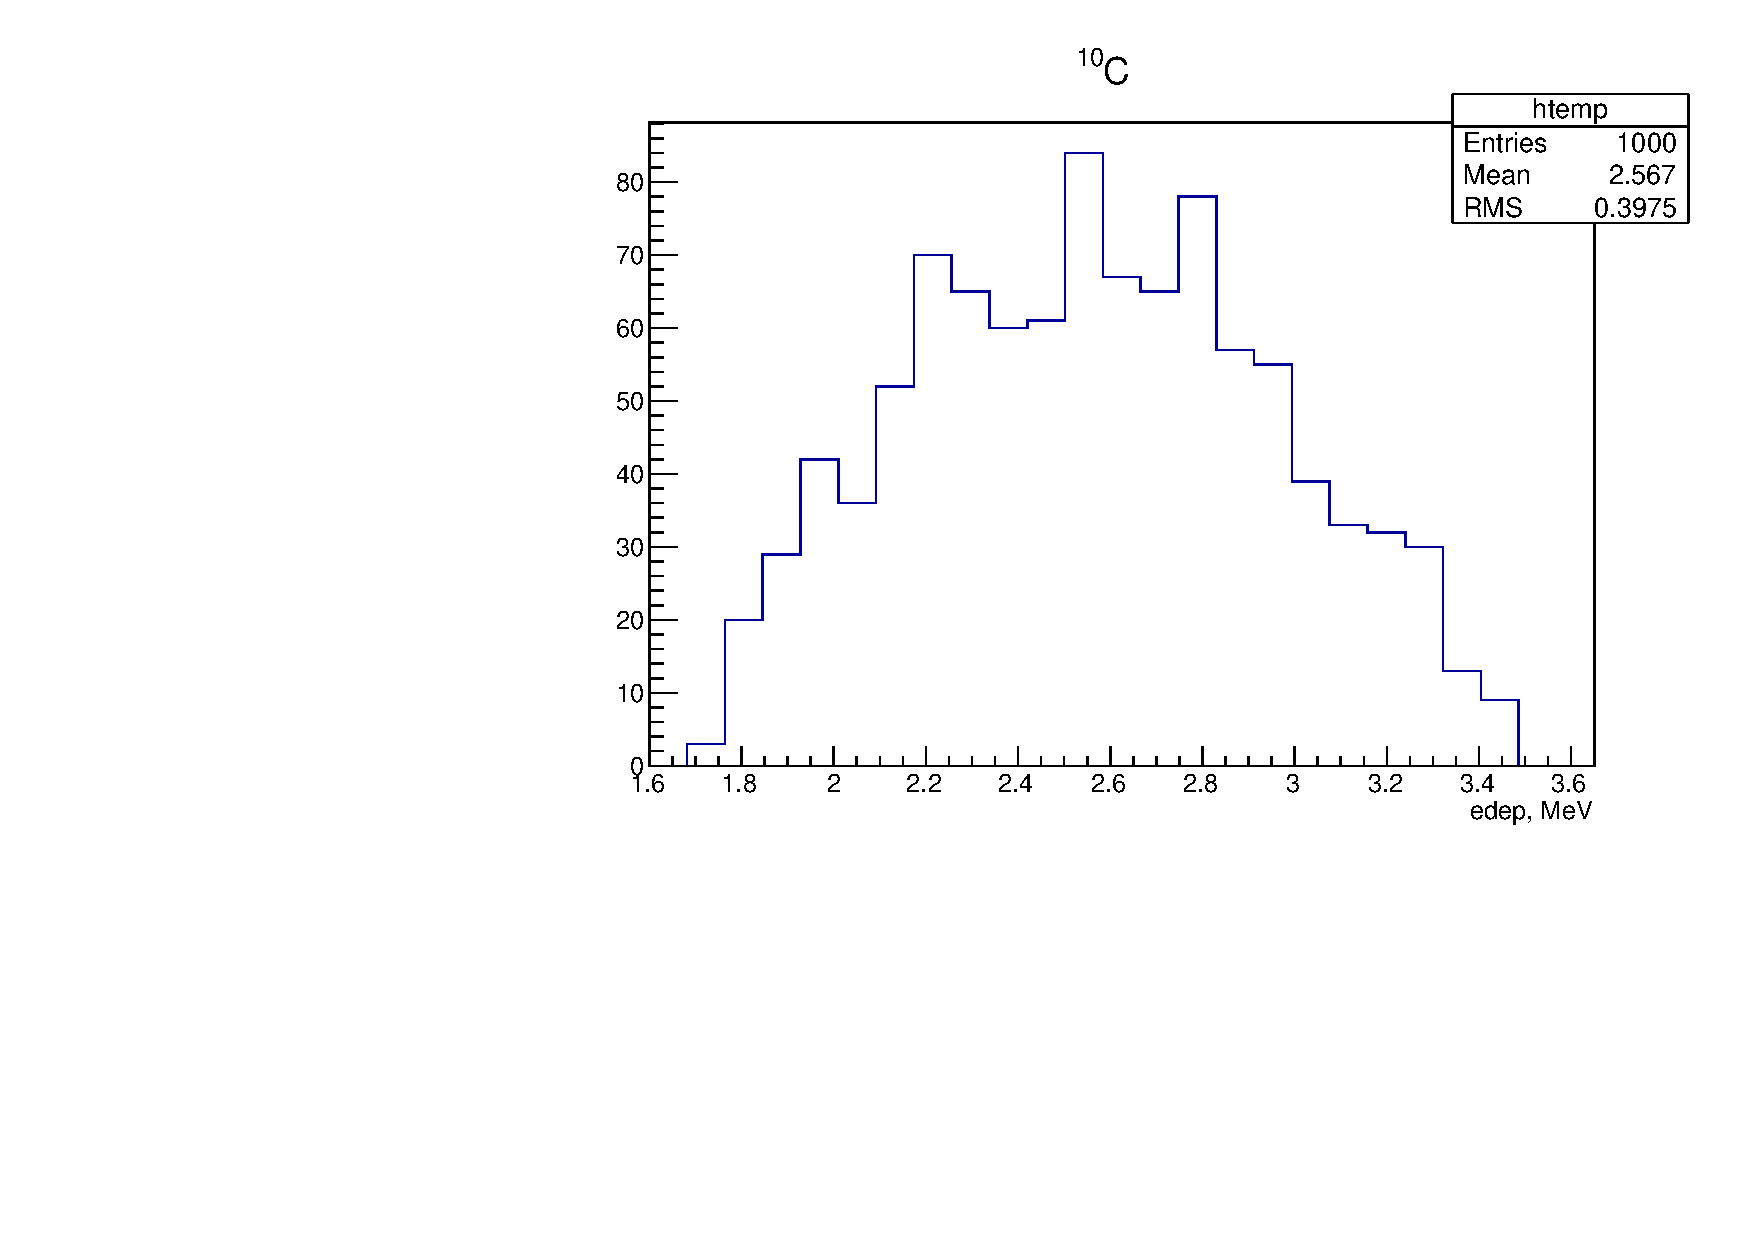
\includegraphics[width=0.95\textwidth]{hEdep_C10.pdf}
  \caption{Energy deposition in $^{10}$C events.}
  \label{fig:Edep_C10}
\end{figure}

\begin{figure}[h]
  \centering
  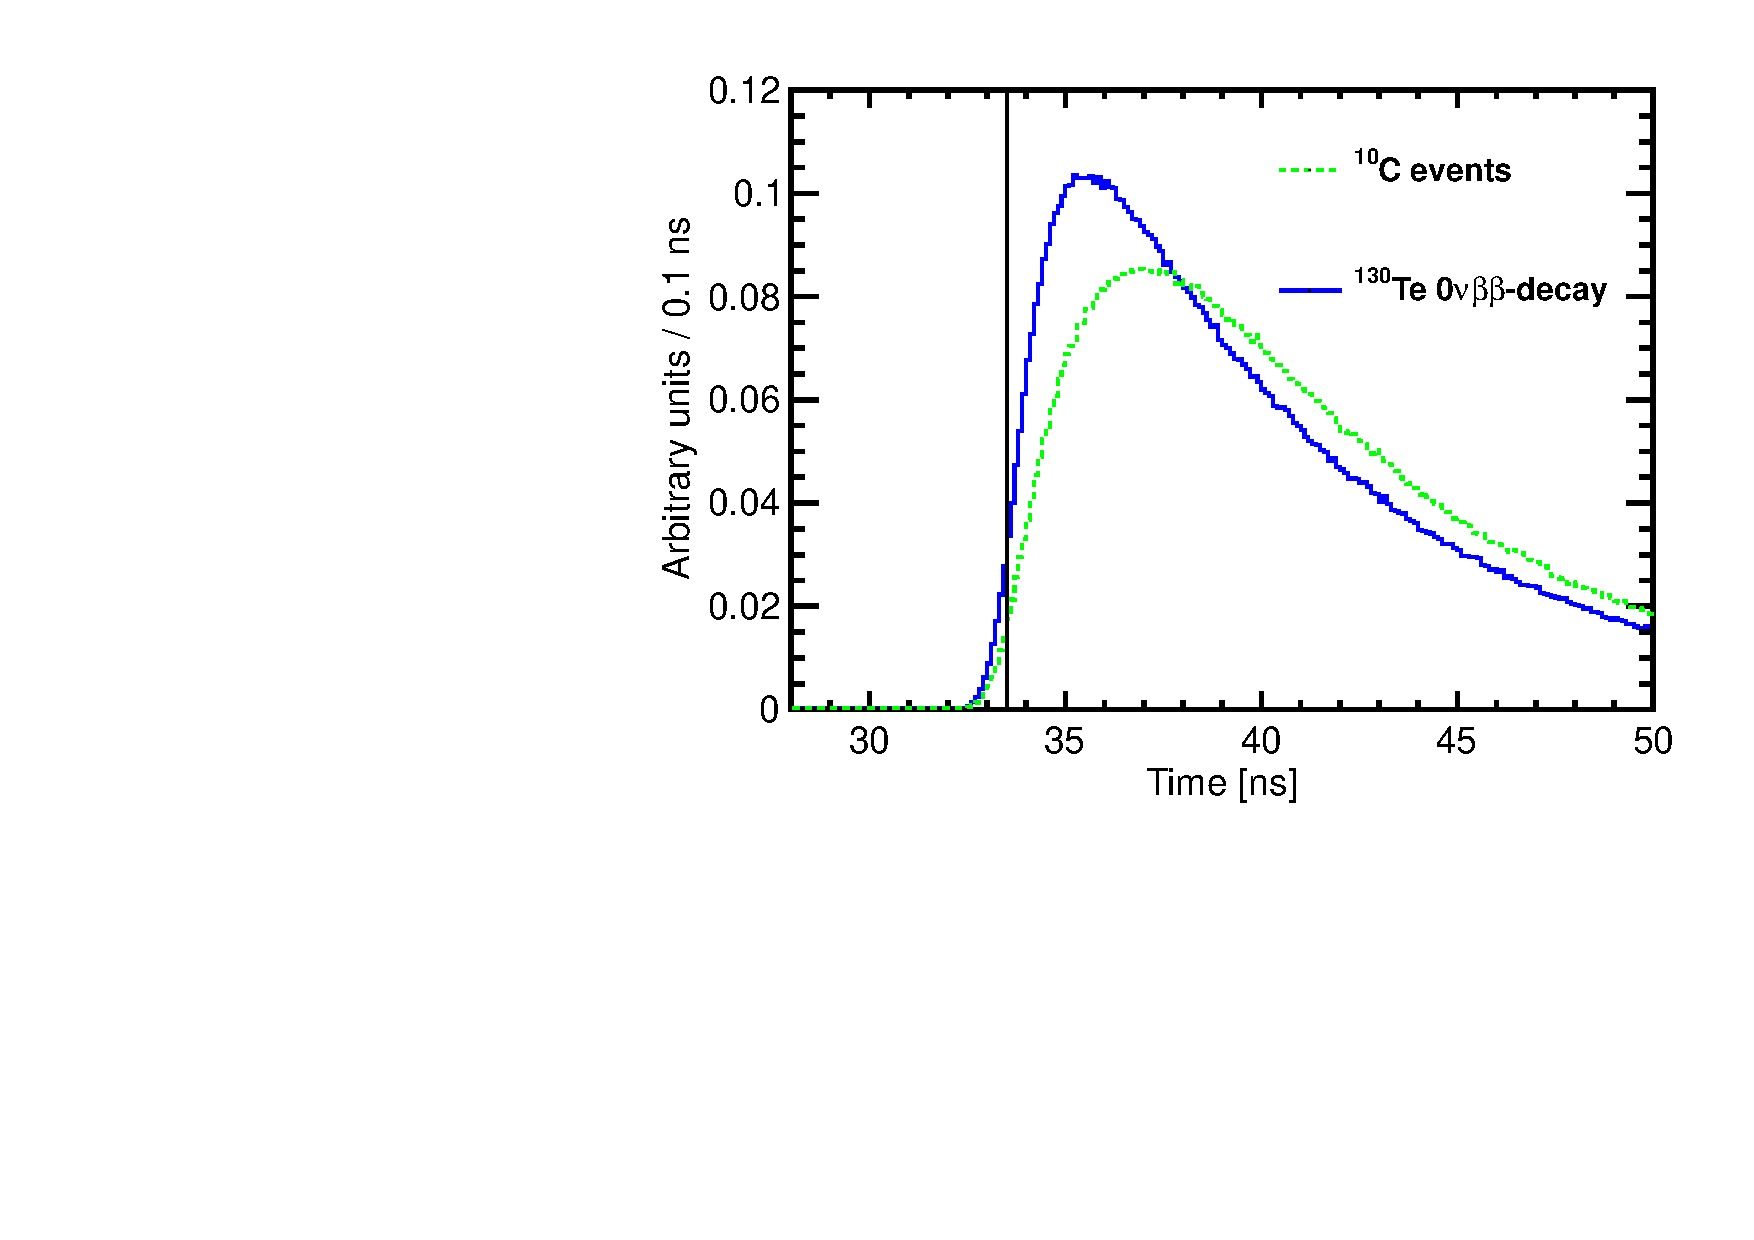
\includegraphics[width=0.45\textwidth]{hT_C10.pdf}
  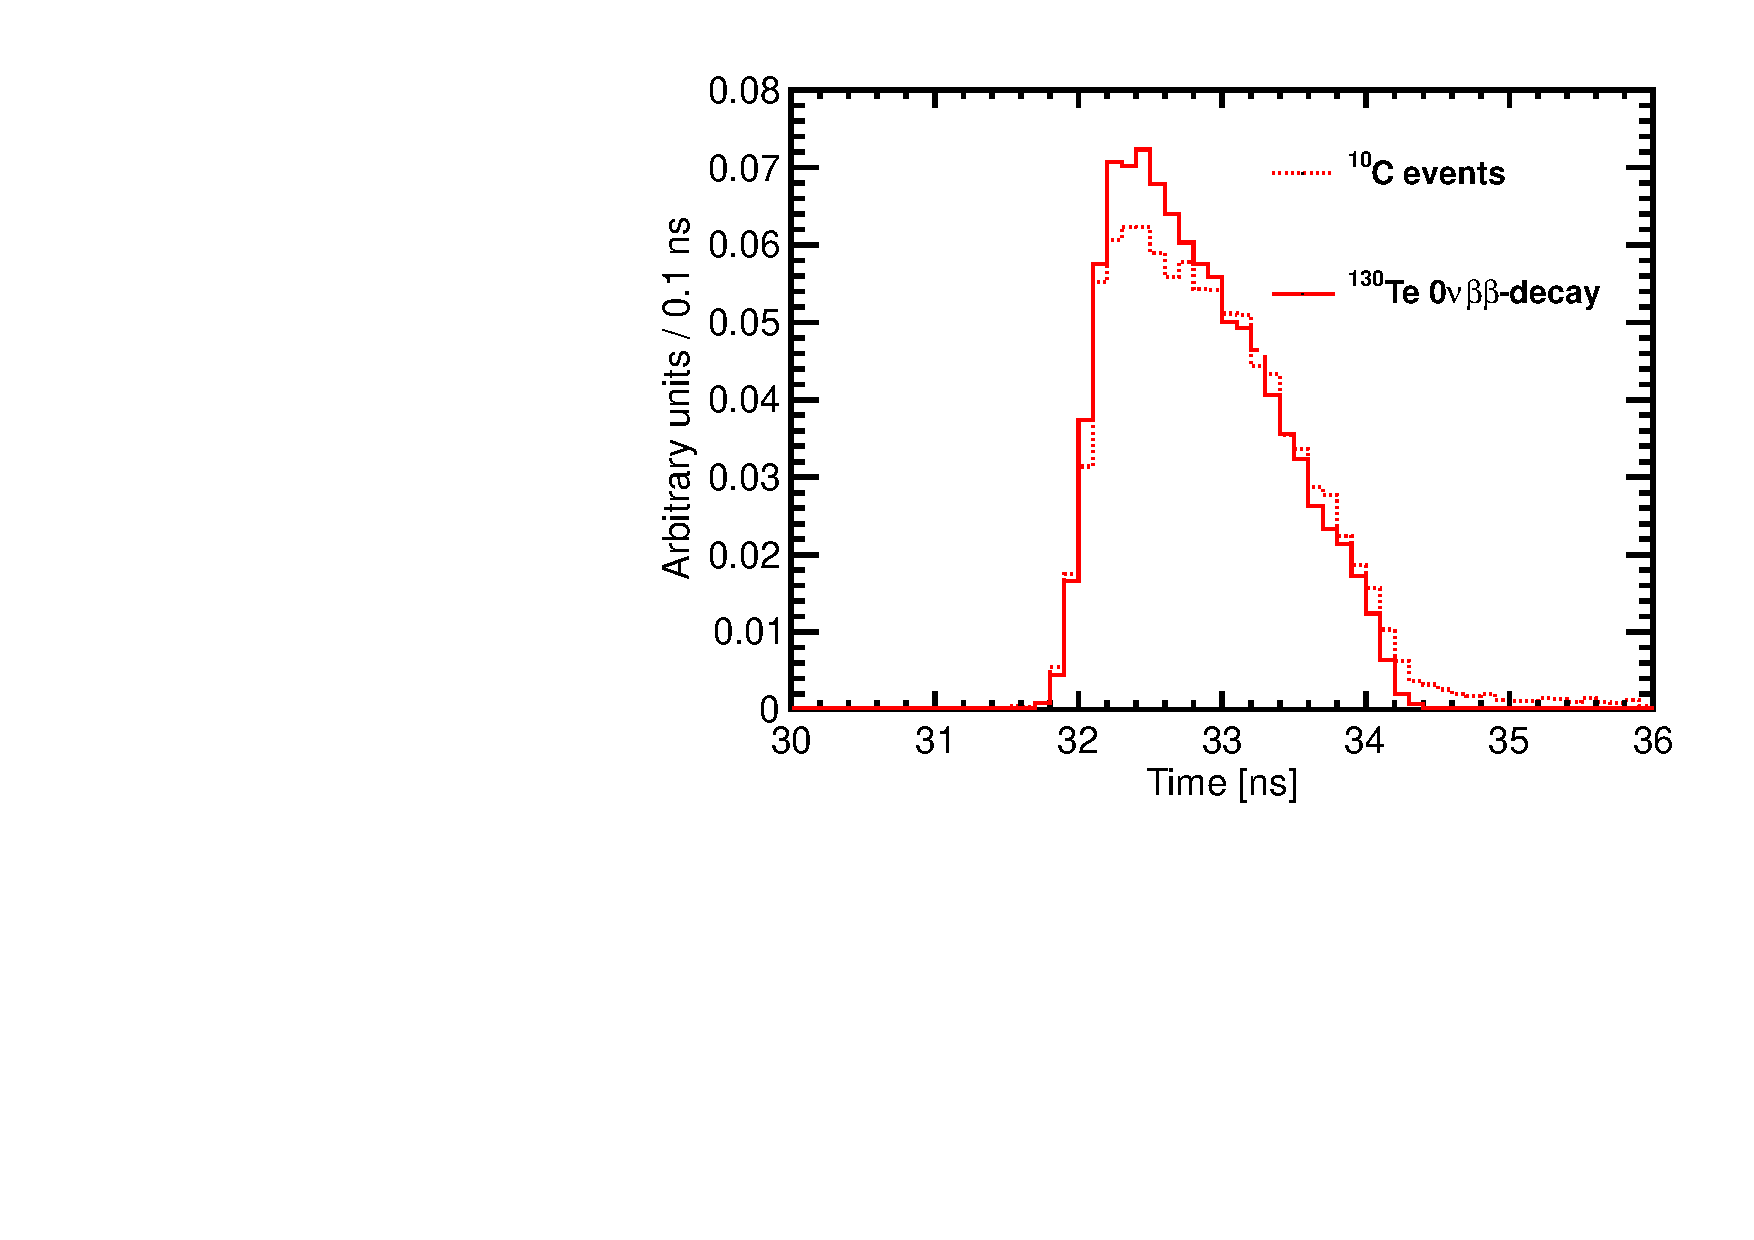
\includegraphics[width=0.45\textwidth]{hTche_C10.pdf}
  \caption{Photo-electron (PE) arrival times after application of the
    photo-detector transit time spread (TTS) of 100~ps for the
    simulation of 1000 0{\nbb} decay events of $^{130}$Te (\emph{solid
      lines}) and $^{10}$C (\emph{dotted lines}) events at the center
    of the detector. All distributions are normalized for shape
    comparison. {\bf Absolute number of PEs per event depends on the
      total energy deposited in the
      detector. Figure~\ref{fig:Edep_C10} shows energy deposited in
      the detector in $^{10}$C events.} \emph{Left:} Scintillation PEs
    arrival time. The black vertical line illustrates a time cut at
    33.5 ns. \emph{Right:} Cherenkov PEs arrival time.}
\label{fig:Arrival_time_C10}
\end{figure}

We note that 98\% of $^{10}$C decays through the excited state of
$^{10}$B(718), which has a half-life time of $\sim$1~ns. Therefore, the
majority of $^{10}$C events have a prompt positron accompanied by a
delayed 0.718~MeV gamma. This delayed gamma affects the PE arrival time
distribution. Figure~\ref{fig:Arrival_time_C10} compares the shape of the
PE arrival time distribution between $^{130}$Te 0{\nbb} decays and
$^{10}$C events. The time profile of the scintillation photons can be used
to separate signal from $^{10}$C events.

\end{comment}

%	!!!!!!!!!!!!!!!!	Commented text ends 	!!!!!!!!!!!!!!!!!!

Comparison of $S_0$ and $S_1$ distributions between 0{\nbb} decay and
$^{10}$C events is shown in Fig.~\ref{fig:S_vs_energy_C10}.

\begin{figure*}[h]
\centering
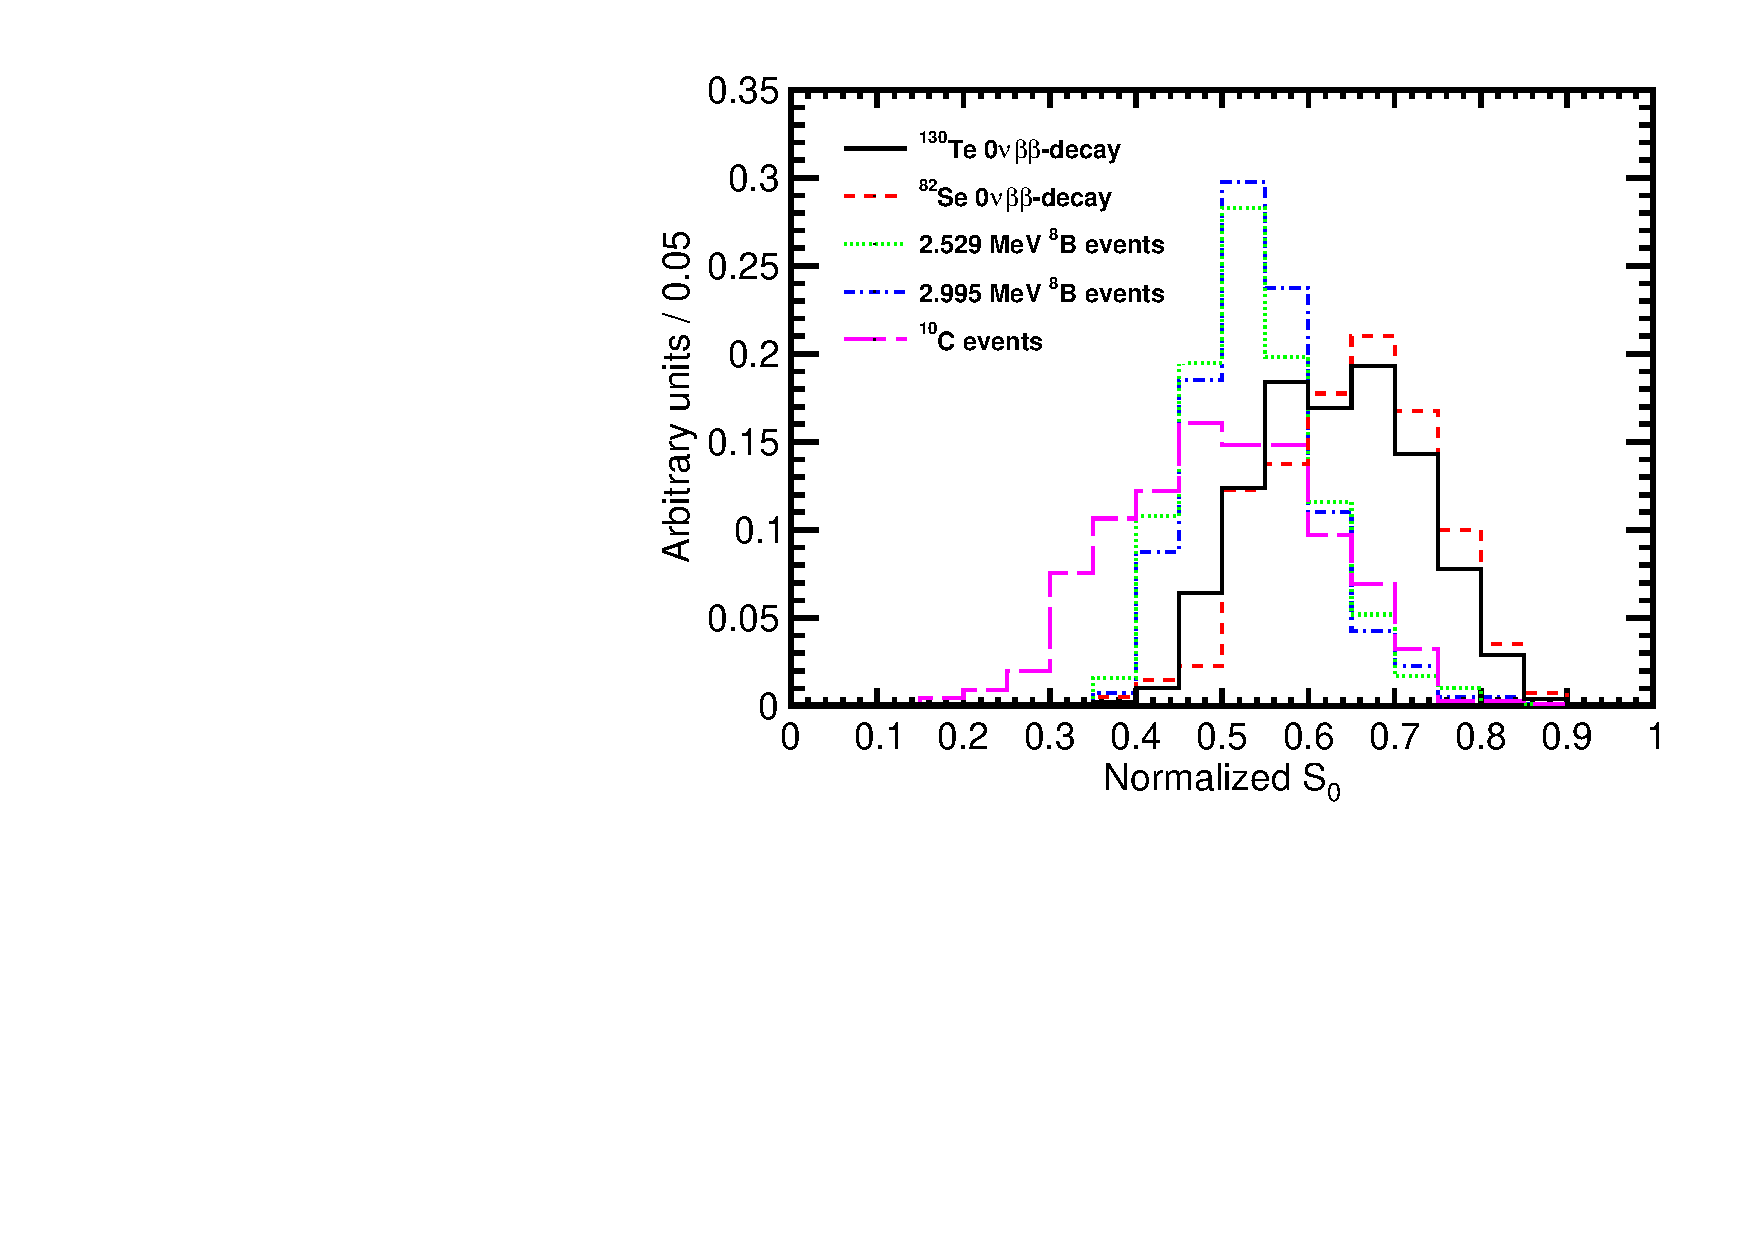
\includegraphics[width=0.49\textwidth]{hS0_C10.pdf}
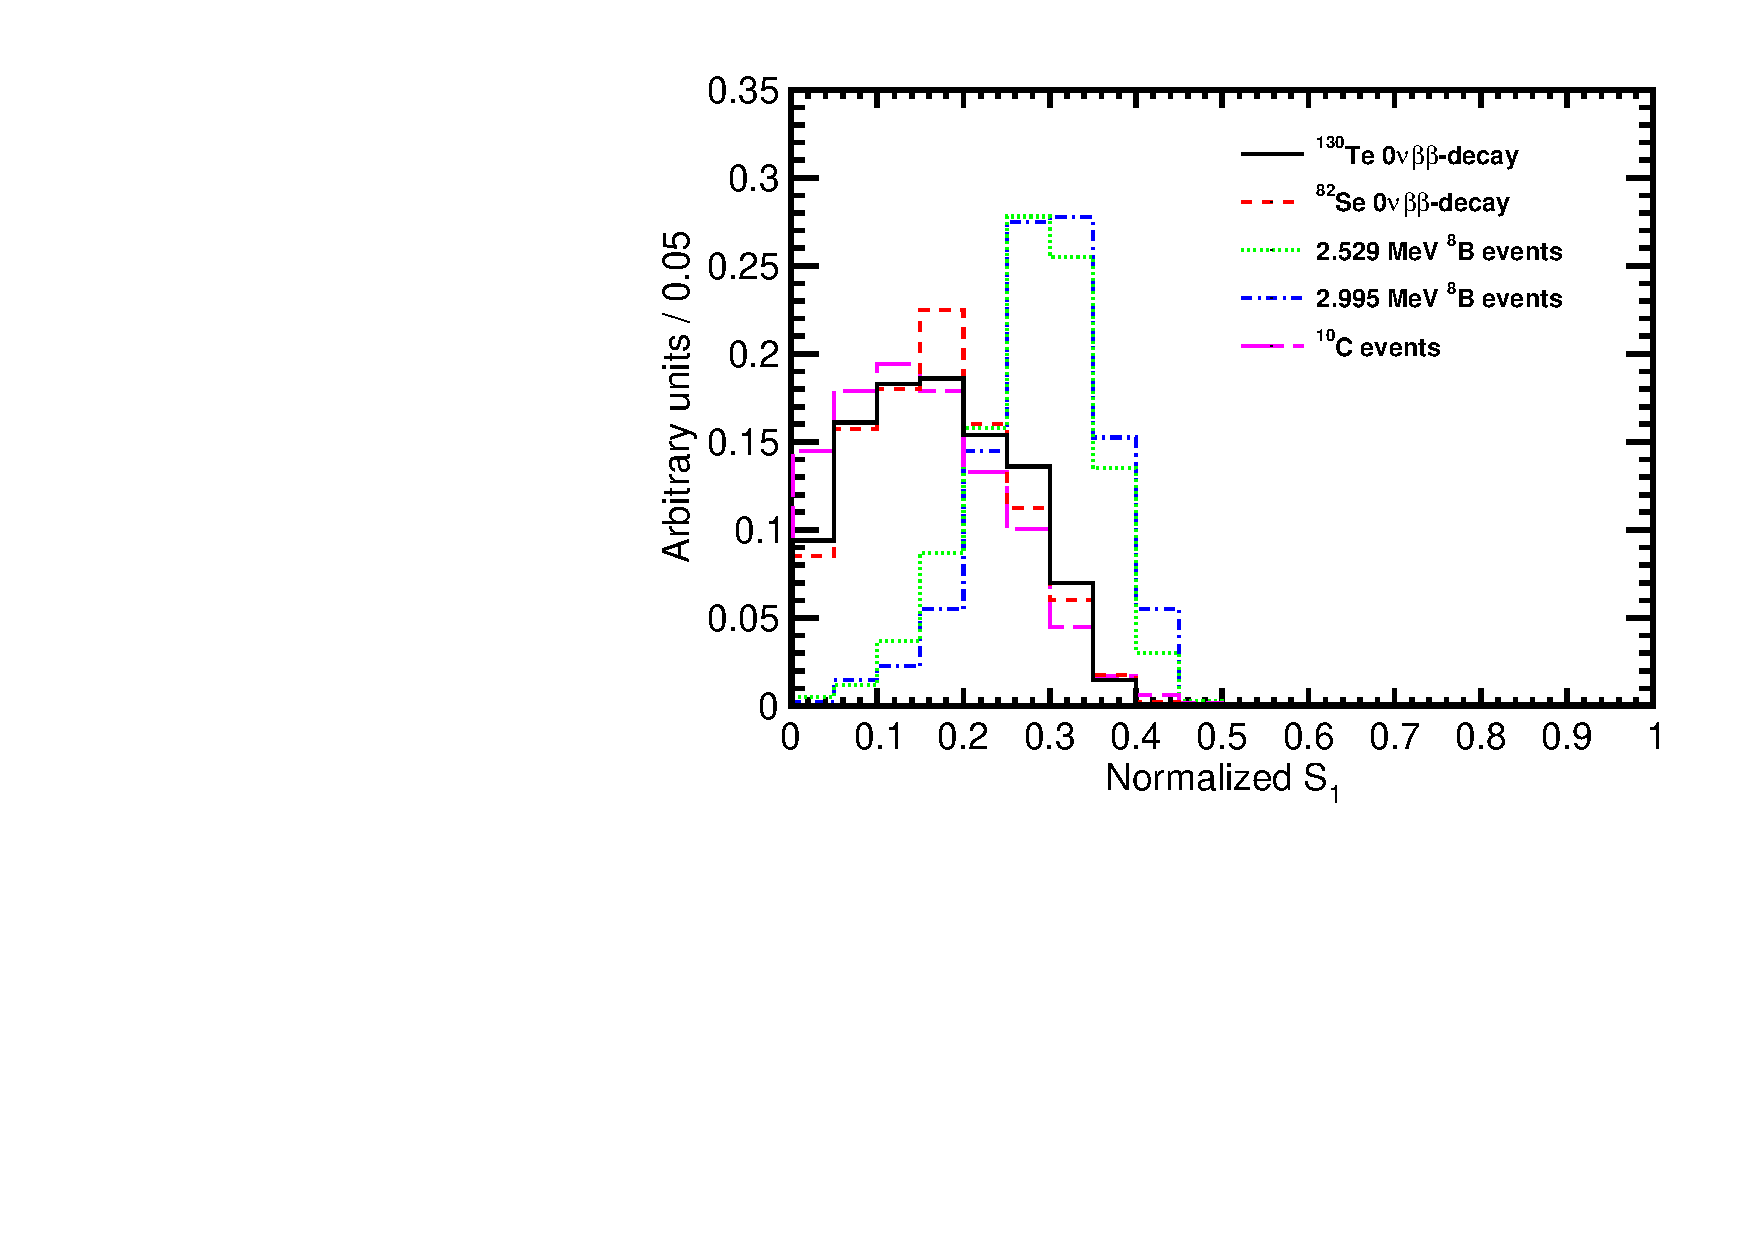
\includegraphics[width=0.49\textwidth]{hS1_C10.pdf}
\caption{$S_0$ (\emph{left}) and $S_1$ (\emph{right}) distributions
  for events with different event topologies. $^{130}$Te, $^{82}$Se 0{\nbb} 
  decays compared with $^{8}$B and $^{10}$C events. The simulation is done 
  for events with the vertex in the center of the detector. $^{8}$B events 
  are implemented as 2.529~MeV or 2.995~MeV electrons with initial direction 
  along $x$-axis. $^{10}$C events are selected in the energy range between 2.1 
  and 2.9~MeV. Perfect vertex reconstruction - true vertex position is used. 
  Time cut of 33.5~ns on the photon arrival time is applied.}
\label{fig:S_vs_energy}
\end{figure*}


\begin{figure}[h]
  \centering
  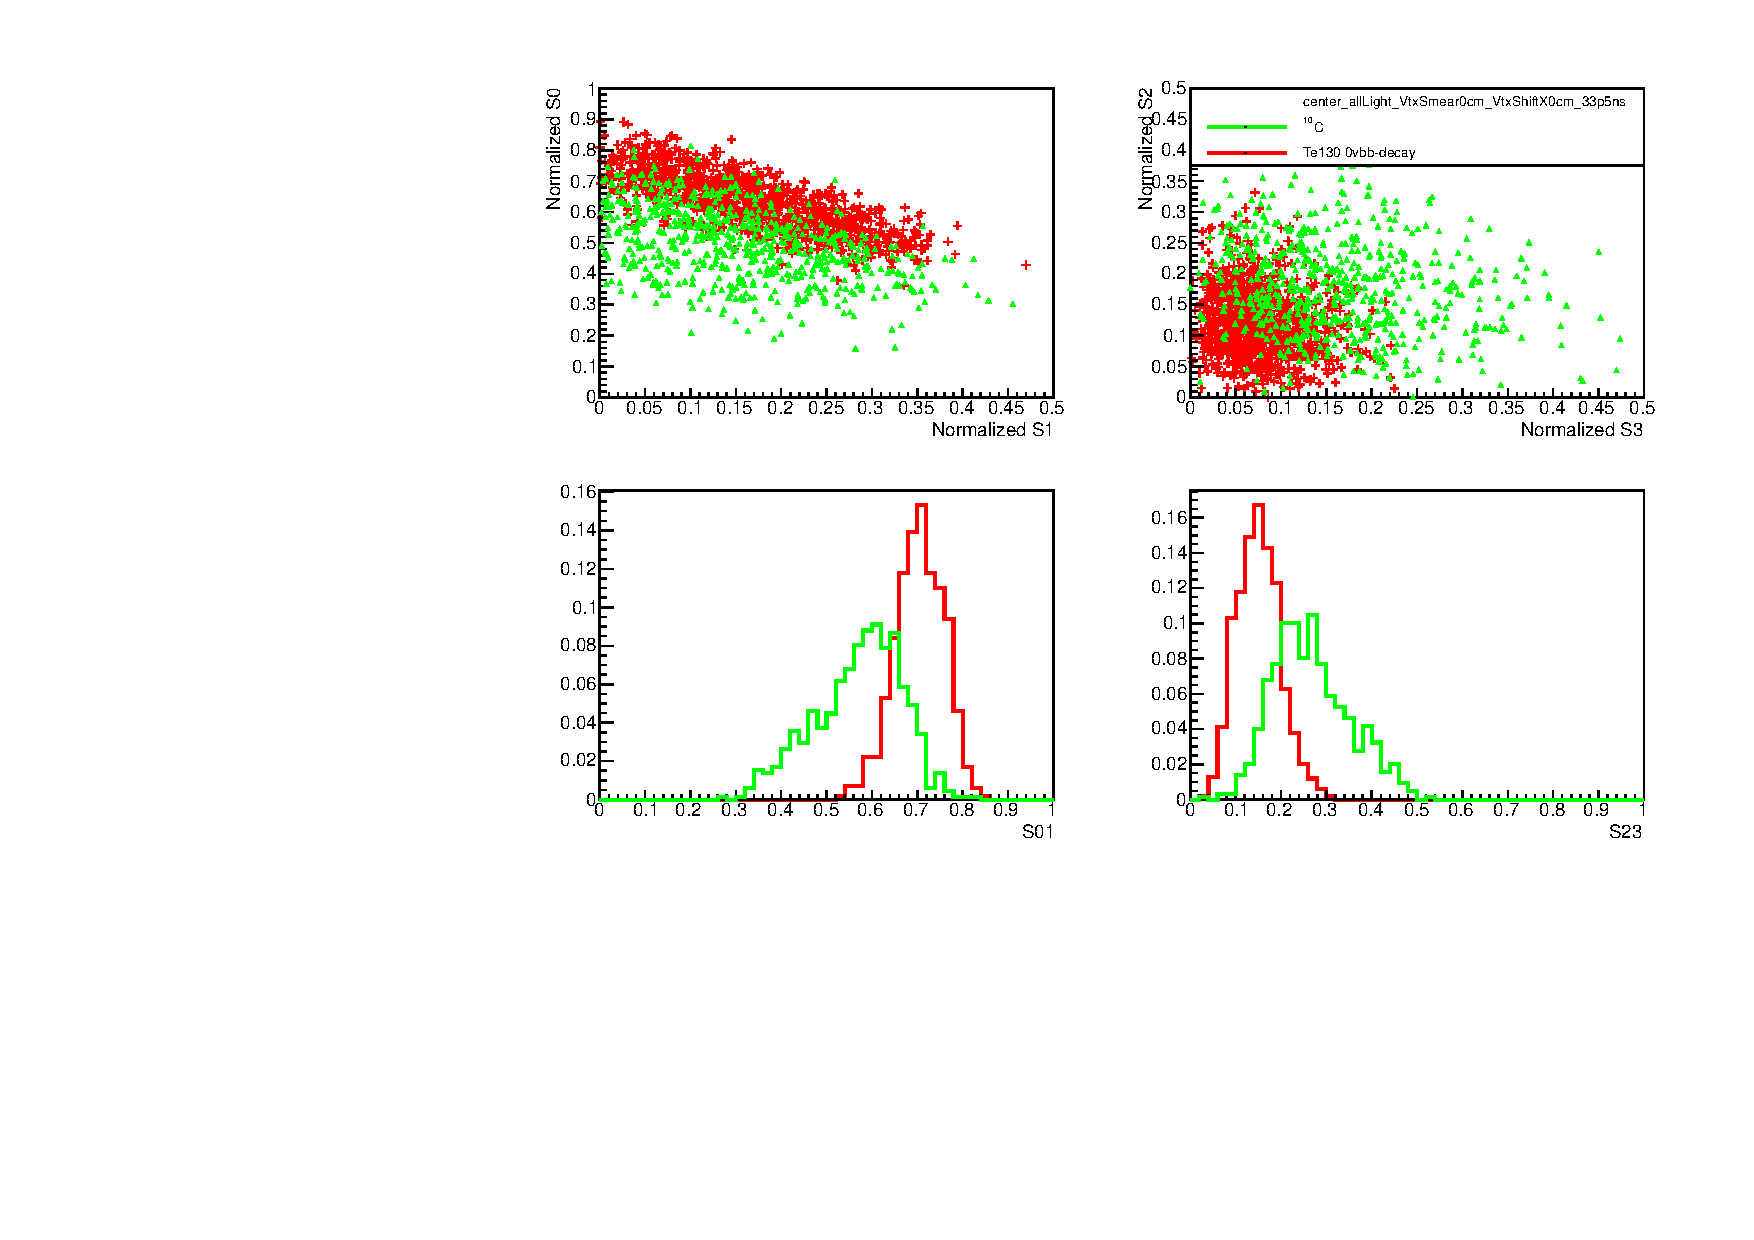
\includegraphics[width=0.95\textwidth]{hSLPlots_C10_allLight_VtxSmear0cm_VtxShiftX0cm_33p5ns_center.pdf}
  \caption{Spherical harmonics comparison between $^{130}$Te 0{\nbb}
    decay signal ($Q=2.529$~MeV) (\emph{red}) and $^{10}$C solar
    neutrinos background (blue) for 1000 simulated events originated
    at the center of the sphere. $^{10}$C with energy deposition
    between 2.1~MeV and 2.9~MeV are considered. Perfect vertex
    reconstruction - true vertex position is used. Time cut of 33.5~ns
    on the photon arrival time is applied. \emph{Top left:} S$_0$
    versus S$_1$ scatter plot. \emph{Top right:} S$_2$ versus S$_3$
    scatter plot. \emph{Bottom left:} Distribution of the
    S$^{C10}_{01}$ variable calculated for signal (\emph{red}) and
    background (\emph{green}). \emph{Bottom right:} Distribution of
    the S$^{C10}_{23}$ variable calculated for signal (\emph{red}) and
    background (\emph{green}).}
  \label{fig:SL_C10_33p5ns_center}
\end{figure}


Comparison of spherical harmonics is shown in
Fig.~\ref{fig:SL_C10_33p5ns_center}. $^{10}$C events are generated at
the center of the detector. True vertex position is used to apply a
33.5~ns time cut to select photons for the spherical harmonics
analysis. The separation is seen in S0 vs S1 and S2 vs S3 scatter
plots. We project both scatter plots to a line that gives maximum
separation (two bottom panels in Fig.~\ref{fig:SL_C10_33p5ns_center}).  
There is enough separation between the distributions to suggest that this analysis can be used to distinguish between 0{\nbb} and $^{10}$C events.

%\section{0{\nbb} decay vs backgrounds from Th and U series}
